%Input preamble
%Style
\documentclass[12pt]{article}
\usepackage[top=1in, bottom=1in, left=1in, right=1in]{geometry}
\parindent 22pt
\usepackage{fancyhdr}

%Packages
\usepackage{adjustbox}
\usepackage{amsmath}
\usepackage{amsfonts}
\usepackage{amssymb}
\usepackage{bm}
\usepackage[table]{xcolor}
\usepackage{tabu}
\usepackage{color,soul}
\usepackage{makecell}
\usepackage{longtable}
\usepackage{multirow}
\usepackage[normalem]{ulem}
\usepackage{etoolbox}
\usepackage{graphicx}
\usepackage{tabularx}
\usepackage{ragged2e}
\usepackage{booktabs}
\usepackage{caption}
\usepackage{fixltx2e}
\usepackage[para, flushleft]{threeparttablex}
\usepackage[capposition=top,objectset=centering]{floatrow}
\usepackage{subcaption}
\usepackage{pdfpages}
\usepackage{pdflscape}
\usepackage{natbib}
\usepackage{bibunits}
\definecolor{maroon}{HTML}{990012}
\usepackage[colorlinks=true,linkcolor=maroon,citecolor=maroon,urlcolor=maroon,anchorcolor=maroon]{hyperref}
\usepackage{marvosym}
\usepackage{makeidx}
\usepackage{tikz}
\usetikzlibrary{shapes}
\usepackage{setspace}
\usepackage{enumerate}
\usepackage{rotating}
\usepackage{tocloft}
\usepackage{epstopdf}
\usepackage[titletoc]{appendix}
\usepackage{framed}
\usepackage{comment}
\usepackage{xr}
\usepackage{titlesec}
\usepackage{footnote}
\usepackage{longtable}
\newlength{\tablewidth}
\setlength{\tablewidth}{9.3in}
\setcounter{secnumdepth}{4}

\titleformat{\paragraph}
{\normalfont\normalsize\bfseries}{\theparagraph}{1em}{}
\titlespacing*{\paragraph}
{0pt}{3.25ex plus 1ex minus .2ex}{1.5ex plus .2ex}
\makeatletter
\pretocmd\start@align
{%
  \let\everycr\CT@everycr
  \CT@start
}{}{}
\apptocmd{\endalign}{\CT@end}{}{}
\makeatother
%Watermark
\usepackage[printwatermark]{xwatermark}
\usepackage{lipsum}
\definecolor{lightgray}{RGB}{220,220,220}
%\newwatermark[allpages,color=lightgray,angle=45,scale=3,xpos=0,ypos=0]{Preliminary Draft}

%Further subsection level
\usepackage{titlesec}
\setcounter{secnumdepth}{4}
\titleformat{\paragraph}
{\normalfont\normalsize\bfseries}{\theparagraph}{1em}{}
\titlespacing*{\paragraph}
{0pt}{3.25ex plus 1ex minus .2ex}{1.5ex plus .2ex}

\setcounter{secnumdepth}{5}
\titleformat{\subparagraph}
{\normalfont\normalsize\bfseries}{\thesubparagraph}{1em}{}
\titlespacing*{\subparagraph}
{0pt}{3.25ex plus 1ex minus .2ex}{1.5ex plus .2ex}

%Functions
\DeclareMathOperator{\cov}{Cov}
\DeclareMathOperator{\corr}{Corr}
\DeclareMathOperator{\var}{Var}
\DeclareMathOperator{\plim}{plim}
\DeclareMathOperator*{\argmin}{arg\,min}
\DeclareMathOperator*{\argmax}{arg\,max}

%Math Environments
\newtheorem{theorem}{Theorem}
\newtheorem{claim}{Claim}
\newtheorem{condition}{Condition}
\renewcommand\thecondition{C--\arabic{condition}}
\newtheorem{algorithm}{Algorithm}
\newtheorem{assumption}{Assumption}
\renewcommand\theassumption{A--\arabic{assumption}}
\newtheorem{remark}{Remark}
\renewcommand\theremark{R--\arabic{remark}}
\newtheorem{definition}[theorem]{Definition}
\newtheorem{hypothesis}[theorem]{Hypothesis}
\newtheorem{property}[theorem]{Property}
\newtheorem{example}[theorem]{Example}
\newtheorem{result}[theorem]{Result}
\newenvironment{proof}{\textbf{Proof:}}{$\bullet$}

%Commands
\newcommand\independent{\protect\mathpalette{\protect\independenT}{\perp}}
\def\independenT#1#2{\mathrel{\rlap{$#1#2$}\mkern2mu{#1#2}}}
\newcommand{\overbar}[1]{\mkern 1.5mu\overline{\mkern-1.5mu#1\mkern-1.5mu}\mkern 1.5mu}
\newcommand{\equald}{\ensuremath{\overset{d}{=}}}
\captionsetup[table]{skip=10pt}
%\makeindex

\setlength\parindent{20pt}
\setlength{\parskip}{0pt}

\newcolumntype{L}[1]{>{\raggedright\let\newline\\\arraybackslash\hspace{0pt}}m{#1}}
\newcolumntype{C}[1]{>{\centering\let\newline\\\arraybackslash\hspace{0pt}}m{#1}}
\newcolumntype{R}[1]{>{\raggedleft\let\newline\\\arraybackslash\hspace{0pt}}m{#1}}



%Logo
%\AddToShipoutPictureBG{%
%  \AtPageUpperLeft{\raisebox{-\height}{
\includegraphics[width=1.5cm]{uchicago.png}}}
%}

\newcolumntype{L}[1]{>{\raggedright\let\newline\\\arraybackslash\hspace{0pt}}m{#1}}
\newcolumntype{C}[1]{>{\centering\let\newline\\\arraybackslash\hspace{0pt}}m{#1}}
\newcolumntype{R}[1]{>{\raggedleft\let\newline\\\arraybackslash\hspace{0pt}}m{#1}}

\newcommand{\mr}{\multirow}
\newcommand{\mc}{\multicolumn}

%\newcommand{\comment}[1]{}

%Other parameters
\newcommand{\noutcomes}{95}
\newcommand{\noutcomesexpp}{357}
\newcommand{\noutcomesexpm}{343}
\newcommand{\noutcomesexpf}{355}
\newcommand{\treatsubsabc}{$75\%$}
\newcommand{\treatsubscarec}{$74\%$}
\newcommand{\treatsubscaref}{$63\%$}

%Counts
%Males
\newcommand{\positivem}{$78\%$}
\newcommand{\positivesm}{$29\%$}

%Females
\newcommand{\positivef}{$78\%$}
\newcommand{\positivesf}{$31\%$}

%Counts, control substitution
%Males
\newcommand{\positivecsnm}{$47\%$}
\newcommand{\positivescsnm}{$15\%$}

\newcommand{\positivecsam}{$79\%$}
\newcommand{\positivescsam}{$29\%$}

%Females
%% no alternative
\newcommand{\positivecsnf}{$84\%$}
\newcommand{\positivescsnf}{$55\%$}

%% alternative
\newcommand{\positivecsaf}{$79\%$}
\newcommand{\positivescsaf}{$33\%$}

%Pooled

%Effects
%Males

%Females
\newcommand{\empf}{$8$}
\newcommand{\yearsedf}{$1.7$}



%Pooled

%CBA
%IRR
%Males
\newcommand{\irrm}{$15\%$}
\newcommand{\irrsem}{$5\%$}

%Females
\newcommand{\irrf}{$9\%$}
\newcommand{\irrsef}{$7\%$}

%Pooled
\newcommand{\irrp}{$13\%$}
\newcommand{\irrsep}{$5\%$}

%BC
%Males
\newcommand{\bcm}{$11.24$}
\newcommand{\bcsem}{$4.60$}

%Females
\newcommand{\bcf}{$2.35$}
\newcommand{\bcsef}{$1.09$}

%Pooled
\newcommand{\bcp}{$5.63$}
\newcommand{\bcsep}{$2.15$}

%NPV streams
%Pooled
\newcommand{\parincomenpvp}{$\$119,346$}

\externaldocument{abc_comprehensivecba_appendix_AA1_2016-08-19a_jbb.tex}
\pagenumbering{roman}

\begin{document}

\begin{titlepage}

\title{\Large \textbf{The Life Cycle Benefits of an Influential Early Childhood Intervention}\thanks{This research was supported in part by the American Bar Foundation; the Pritzker Children's Initiative, the Buffett Early Childhood Fund, National Institutes of Health grants NICHD R37HD065072, NICHD R01HD54702, NIA R24AG048081, P30AG024968, an anonymous funder, Successful Pathways from School to Work, an initiative of the University of Chicago's Committee on Education funded by the Hymen Milgrom Supporting Organization, and the Human Capital and Economic Opportunity Global Working Group, an initiative of the Center for the Economics of Human Development, affiliated with the Becker Friedman Institute for Research in Economics, and funded by the Institute for New Economic Thinking. The views expressed in this paper are solely those of the authors and do not necessarily represent those of the funders or the official views of the National Institutes of Health. Collaboration with Yu Kyung Koh, Sylvi Kuperman, Stefano Mosso, Rodrigo Pinto, and Anna Ziff on related work has strengthened the analysis in this paper. Collaboration with Bryan Tysinger on adapting the Future America Model was invaluable and is gratefully acknowledged. For helpful comments, we thank St\'{e}phane Bonhomme, Fl\'{a}vio Cunha, Steven Durlauf, Azeem Shaikh, Matthew Tauzer, and Ed Vytlacil. For information on the implementation of the Carolina Abecedarian Project and assistance in data acquisition, we thank Peg Burchinal, Carrie Bynum, Frances Campbell, and Elizabeth Gunn. For information on childcare in North Carolina, we thank Richard Clifford and Sue Russell. The Web Appendix for this paper can be found at \url{http://cehd.uchicago.edu/ABC_CARE}.}}

\author{
Jorge Luis Garc\'{i}a\\
The University of Chicago \and
James J. Heckman \\
American Bar Foundation \\
The University of Chicago \and
Andr\'{e}s Hojman\\
The University of Chicago \and
Duncan Ermini Leaf \\
University of Southern California \and
Mar\'{i}a Jos\'{e} Prados \\
University of Southern California \and
Joshua Shea \\
The University of Chicago \and
Jake C. Torcasso\\
The University of Chicago}
\date{First Draft: January 5, 2016\\ This Draft: \today}

\maketitle

\end{titlepage}

\singlespacing

\begin{abstract}
This paper estimates the diverse array of life cycle benefits of an influential early childhood program targeted to disadvantaged children and their families. The program is a prototype for numerous current interventions around the world. It has substantial beneficial long-term effects on (a) health and the quality of life, (b) the earnings of participants, (c) the earnings and education of their mothers through subsidizing childcare, (d) crime, and (e) education. There are pronounced benefits for both genders, with more substantial monetized benefits for boys. The overall rate of return is a statistically significant 13\% per annum with a benefit/cost ratio of 5.6, even after accounting for the welfare costs of taxation to finance the intervention. Estimates are robust to a variety of sensitivity analyses.
\end{abstract}

\noindent \textbf{Keywords}: Health, childcare, crime, randomized trials, early childhood education, gender differences in responses to interventions \\
\noindent \textbf{JEL codes}: J13, I28, C93

\clearpage

\tableofcontents
\listoffigures
\listoftables

\clearpage

\doublespacing

\setcounter{page}{0}
\pagenumbering{arabic}

\noindent Outline of the paper

\begin{enumerate}[(1)]
\item Intense and growing interest in early childhood programs to promote social mobility and economic/social advantage
\item ABC/CARE
    \begin{enumerate}[(a)]
    \item Targets disadvantaged kids
    \item Starts early (8 weeks)/intensive
    \item Prototype for many successor programs currently in place around the world
        \begin{enumerate}[(i)]
        \item IHDP
        \item Early Head Start
        \item Sparling's list (Australia)
        \end{enumerate}
    \item Many children eligible for it in U.S. (19\% of all African-American children)
    \item Documented to have health benefits (not previously accounted and other benefits (Campbell))
    \item Childcare costs:
        \begin{enumerate}[(i)]
        \item Wage growth of women (sustain according to Gladden and Taber)
        \item Leisure foregone
        \item Educational attainment
        \item Costs of inadequate childcare (what is next best)
        \end{enumerate}
    \end{enumerate}
\item Multiple benefits of the program --- goal is to chronicle benefits and place them in a common metric
    \begin{enumerate}[(a)]
    \item Organize by category
    \item Look at benefits
    \item Aggregate benefits
    \end{enumerate}
\item Costs
    \begin{enumerate}[(a)]
    \item Fresh examination of costs: new primary sources
    \item Tax costs (if publicly funded) --- deadweight burden
    \end{enumerate}
\item Evaluation through age 34
    \begin{enumerate}[(a)]
    \item Account for substitution bias
    \item Vectors of outcomes
    \item Deal with multiple outcomes
        \begin{enumerate}[(i)]
        \item Step-down
        \item Counts
        \item CBA
        \end{enumerate}
    \end{enumerate}
\item CBA requires projecting future benefits and costs
    \begin{enumerate}[(a)]
    \item Previous approaches: \emph{ad hoc} (use a test score gain and impute earnings) Chetty et al./Kline and Walters
    \item We merge data from multiple sources on earnings, health costs, crime, childcare savings, quality of life
    \item Account for sampling uncertainty
    \item Sensitivity analysis for cases where there is some uncertainty but not quantifiable
    \end{enumerate}
\item Main findings: differ by gender
    \begin{enumerate}[(a)]
    \item Substantial monetary benefits for health and QALY (primarily for men)
    \item Childcare and earnings benefits (link childcare to child benefits)
    \item Crime (for men)
    \item Earnings gains (both)
    \item Education (primarily women)
    \item Effects on IQ
    \end{enumerate}
\end{enumerate}

\clearpage

\section{Introduction}

This paper estimates the diverse array of life cycle benefits of an intensive and influential early childhood program that starts in the first weeks of life and targets disadvantaged children. Different approaches designed to characterize the numerous benefits of the program all agree that the program has a substantial impact on the life outcomes of participants. Monetizing benefits and costs across multiple domains in a benefit-cost analysis produces a single policy-relevant and economically interpretable summary of the program. It has a rate of return of 13\% per annum and a cost/benefit ratio of 5.6. 

Our analysis contributes to a growing literature on the benefits of early interventions for disadvantaged children.\footnote{See, e.g., \cite{Currie_2011_AER} and \cite{Elango_Hojman_etal_2016_Early-Edu}.} Long-term evidence on their effectiveness is surprisingly limited.\footnote{The major source of evidence is from the Perry Preschool Program (see \citealp{Schweinhart_Montie_ea_2005_BOOKlifetime} and \citealp{Heckman_Moon_etal_2010_RateofReturn,Heckman_Moon_etal_2010_QE}), the ABC/CARE programs (\citealp{Ramey_Campbell_etal_2000_ADS,Ramey-etal_2012-ABC}), and IHDP (\citealp{Gross_Spiker_etal_1997_BOOKHelpinglowbirth,Duncan_Sojourner_2013_JHR}) \textbf{[Typist: Professor, I could not find her on the list of lecturers for the Richard T. Ely lecture---I have removed the ``chapter 1'' part of the reference]}. IHDP was inspired by ABC/CARE \citep[][]{Gross_Spiker_etal_1997_BOOKHelpinglowbirth}.} For want of long-term followup data, many studies of early childhood interventions report outcomes at early ages using a limited set of outcomes like IQ or scores on school readiness measures.\footnote{See, e.g., \cite{Kline_Walters_2014_EvaluatingPublicPrograms} and \cite{Weiland_2013_CD_Impacts-of-Pre-K}.} Yet it is the long-term costs and benefits that are relevant to policy analysis.

This paper analyzes a diverse array of \emph{long-term} benefits from two virtually identical early childhood interventions implemented in sequential order in North Carolina. Both are evaluated by the method of random assignment. The programs are the Carolina Abecedarian Project (ABC) and the Carolina Approach to Responsive Education (CARE), henceforth ABC/CARE. These programs were launched in the early 1970s and have long-term follow-ups through age 34. We analyze their impacts on a variety of life-relevant outcomes such as health, the quality of life, participation in crime, earnings, IQ, schooling, and the subsidy of the mother's employment through subsidizing childcare costs of mothers.

The program starts early (at 8 weeks) and engages participants to age 5. Evidence from these programs is relevant for today's policy discussions because their main features are used in a variety of programs currently in place around the world.\footnote{Programs inspired by ABC have been and are being launched around the world. See \citet{Sparling_2010_Highlights} and \citet{Ramey_Ramey_Lanzi_2014_Interventions} for a list of programs related to and based on ABC/CARE. The names of the programs with years launched and locations in parentheses are: IHDP---eight different cities around the U.S. \citep{Spiker-etal_1997_Helping}; Early Head Start and Head Start in the U.S. \citep{Schneider_McDonald-eds_2007_Scale-Up_Vol-1}; John's Hopkins Cerebral Palsy Study in the U.S. \citep{Sparling_2010_Highlights}; CLIO study in the U.S. \citep{Sparling_2010_Highlights}; Massachusetts Family Child Care Study \citep{Collins_etal_2010_Massachusetts-Study}; Healthy Child Manitoba Evaluation \citep{Healthy_Child_Manitoba_2015_Starting-Early}; Abecedarian Approach within an Innovative Implementation Framework \citep{Jensen_Nielsen_2016_ABC-Programme-Pilot}; and Building a Bridge into Preschool in Remote Northern Territory Communities in Australia \citep{UMonash_Dataset_2015_URL}. Educare programs are based on ABC/CARE \citep{Educare_2014_Research_Agenda,Yazejian_Bryant_2012_Educare}.} Today, roughly 19\% of all African-American children would be eligible for the program.\footnote{33\% of African American children were eligible in 1972 \citep{Garcia_2016_National-Implementation-ECI}.}

Summarizing the benefits of a program with a diverse array of outcomes across many domains and periods of life is challenging. We use a variety of methodologies to characterize its benefits. Instead of just reporting individual treatment effects by category, our benefit/cost analysis accounts for all program components, inclusive of the welfare cost of taxes to publicly finance these programs.\footnote{\cite{Barnett_Masse_2002_benefitcost,Barnett_Masse_2007_EER} present a cost/benefit analysis for ABC for outcomes through age 21, before many benefits are realized. They report a benefit/cost ratio of 2.5, but give no standard error for their estimate. They do not disaggregate by gender. For want of the data collected on health at age 34, they do not account for health benefits. They use self-reported crime data (unlike the police record data later collected that we analyze) and ignore the welfare costs of financing the program. We use cost data from a variety of primary sources not available to them.} Benefit/cost ratios are economically interpretable, policy-relevant summaries of the full impact of the program, which we disaggregate into interpretable components by category.

A fundamental problem facing the evaluation of any human capital program is assessing future benefits of the program not yet surveyed.\footnote{\cite{Mincer_Polachek_1974_JPE} address this problem using a sympathetic cohort approach. See \cite{Heckman_Lochner_etal_2008_JHC}.} We address this problem by combining information from multiple panel data sources on our numerous outcomes to project benefits and costs over the lifetimes of participants.\footnote{See, e.g., \citealp{Ridder_Moffitt_2007_hbk_metricsdata} for a valuable discussion of data pooling methods.} We account for sampling uncertainty in pooling data and conduct sensitivity analyses for components where sampling uncertainty is not readily quantified. Our approach to pooling multiple data sets and analyzing blocks of outcomes is of interest in their own right as a template for evaluating other programs with numerous outcomes, although this is not primarily a paper on methodology.

An important contribution of this paper is our analysis of the long-run benefits of the intervention. We estimate the savings in life cycle medical costs and improvements on the quality of life.\footnote{\cite{Campbell_Conti_etal_2014_EarlyChildhoodInvestments} show the substantial adult (age 34) health benefits of ABC but do not present a cost/benefit analysis of their results.} We also find substantial childcare benefits that promote the work of mothers of participating children. There are substantial adult (age 34) benefits in terms of reduced crime, gains in life cycle earnings, and educational attainment.\footnote{The rate of return is a statistically significant 13\% with an associated benefit/cost ratio of 5.6.} \textbf{[JJH: Jorge, what do we have on special education, etc?] [JLG: we do have special education and grade repetition and it is part of the benefits of the program. There is a reduction. We are quantifying it. It's part of the benefits we quantify as part of education (most of education is costs because people in treatment got more to school. Special education and grade repetition are a benefit.) We do not have it as a separate item because it is small.]}

Figure 1 summarizes the main findings of the paper. It displays the program costs and benefits for a pooled sample of participants: Costs are substantial, as has frequently been noted in public policy discussions.\footnote{\cite{Whitehurst_2014_Senate_Testimony}.} But so are benefits. Breaking down the benefits by category we find substantial benefits for the labor income of participants and their mothers, reduced medical costs, enhanced quality of life, and reduced crime.

\begin{sidewaysfigure}[H]
\caption{Life-cycle Net Present Value of Main Components of the CBA, Pooled Sample of Males and Females}
\label{figure:npvs}
\centering
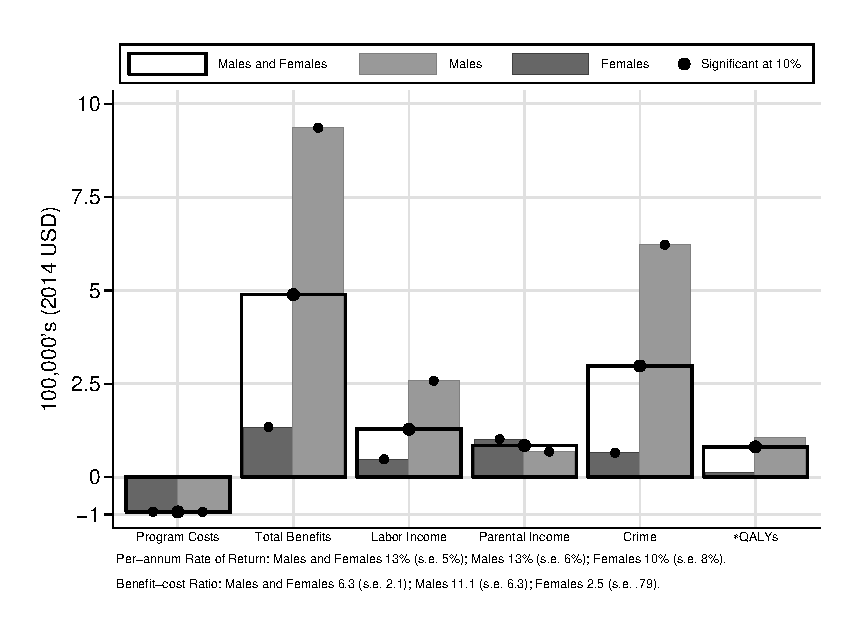
\includegraphics[width=.8\columnwidth]{output/abccare_npvssumm.eps}
\floatfoot{
\footnotesize
Note: This figure displays the life-cycle net present values of the main components of the cost-benefit analysis of ABC/CARE.  By ``net” we mean that each component represents the total value for the treatment group minus the total value for the control group. Program costs refers to the total cost of implementing ABC/CARE. Total net benefits represents the total net benefits of \textit{all} the components we consider. Labor income represents total individual labor income from ages 20 to the retirement of program participants. Parental income represents total parental labor income of the parents of the program participants from when the participants were ages 0 to 15. Crime is the total cost of crime (judiciary plus victimization). QALYs refers to the quality-adjusted life years gain due to better health conditions through age 79. Total medical costs accounts for both private and public medical costs from ages 15 to 79. Costs of education represent the total costs of education of the individual from ages 6 to 26 and \textit{include any costs from special education and grade retention.}
}
\end{sidewaysfigure}

\textbf{[JJH: Jorge, please make a coherent figure for the program overall. What are control substitutions and benefits? Where is reduced special education? At base of table please place definition of each item. What is ``control substitution''? Please be clear. Edit down --- figure too busy. Just present the overall numbers (stay at home and alt preschool)] [Typist: Jorge is working on this paper]}

The rest of the paper justifies this figure and interprets it. We build up to it in the following way. Section~\ref{section:background} discusses main features of ABC/CARE. Many details are relegated to a Web Appendix. Section~\ref{section:methodology} discusses the methodological challenges faced in evaluating the program. There are many outcomes measured across multiple stages of the life cycle and across many domains. 

To address this issue, we use three main methodologies: (a) step down multiple hypothesis testing procedures following \cite{Romano_Wolf_2005_JASA}, reporting blocks of outcomes and adjusting $p$-values for the multiplicity of reported outcomes to avoid cherry-picking of ``significant'' results (see, e.g., \citealp{Heckman_Moon_etal_2010_QE}); (b) combining functions that summarize the \emph{number} of beneficial outcomes (as well as the number of statistically significant beneficial outcomes) within blocks of outcomes and overall. This gives a convenient summary of the mass of evidence in favor of program effects. Our principal too is (c), cost/benefit analysis, which monetizes the costs and benefits associated with outcomes. We also disaggregate benefits by categories as depicted in Figure 1. 

A second methodological challenge is control group substitution bias.\footnote{See \cite{Heckman_1992_randomization}, \cite{Heckman_Hohmann_etal_2000_QJE}, and \cite{Kline-Walters_2016_QJE}.} Roughly 70\% of our experimental control groups take some form of alternative preschool at least some of the time. We define and estimate counterfactuals corresponding to (i) treatment versus the next best, (ii) treatment versus stay at home, and (iii) treatment versus alternative preschool. Doing so highlights importance of the program compared to each alternative. 

Section~\ref{section:results} reports and discusses the estimates of treatment effects, combining function and benefit/cost ration. Estimates from the three methodologies agree. There are substantial benefits that differ by gender. Women benefit across more domains measured in terms of treatment effects. The monetized value of the treatment effects is greater for men. This is largely driven by the health benefits and reduction in crime for boys. Section~\ref{section:conclusion} concludes.

\section[Background and Data Sources]{Background and Data Sources\footnote{This section of the paper is based on joint work with Sylvi Kuperman. We expand it  in Appendix~\ref{appendix:background} and Appendix~\ref{app:programcosts}.}} \label{section:background}

\subsection{Overview}

ABC and CARE targeted disadvantaged children in Chapel Hill/Durham, North Carolina.\footnote{They were designed and implemented by researchers at the Frank Porter Graham Center of the University of North Carolina in Chapel Hill.} Appendix~\ref{appendix:background} describes these programs in detail. Here, we summarize their main features. The goals of the interventions were to remediate disadvantages that hindered early-life development by enhancing the early-life skills of at-risk population. This was done by i) supporting language, motor, and cognitive development; (ii) minimizing high-risk behaviors; and (iii) developing socio-emotional competencies considered crucial for school success including task-orientation, communicative competence, independence, and pro-social behavior.\footnote{\citet{Ramey_Collier_etal_1976_CarolinaAbecedarianProject, Ramey_etal_1985_Project-CARE_TiECSE, Sparling_1974_Synth_Edu_Infant_SPEECH, Wasik_Ramey_etal_1990_CD, Ramey-etal_2012-ABC}.} These programs evolved with experience.\footnote{ \citet{Ramey-etal_1975_AJoMD, Finkelstein_1982_Day_Care_YC, McGinness_1982_Language-Poverty-Child,Haskins_1985_CD}.}

ABC/CARE learning programs were influenced by key developmental theorists, including Bowlby, Piaget, and Vygotsky.\footnote{\citet{Sparling_1974_Synth_Edu_Infant_SPEECH,Mcginness_1981_Developing,abc2014-2015interviews}.} The program provided individualized treatment. Infant caregivers recorded child observations on progress charts and adapted learning activities every 2 to 3 weeks for each treated subject.\footnote{\citet{Ramey_Collier_etal_1976_CarolinaAbecedarianProject,Campbell_Ramey_1994_CD}.} Environments were organized to promote pre-literacy and access to a rich set of learning tools.\footnote{The ``Learningames'' approach was implemented by infant and toddler caregivers in 1:1 child-adult interactions. Each ``Learningames'' activity stated a developmentally-appropriate objective, the necessary materials, directions for teacher behavior, and expected child outcome.} The curriculum emphasized active learning experiences, dramatic play, and pre-academics. At later ages (3 through 5), the program increasingly structured the development of pre-academic skills and ``socio-linguistic and communicative competence.''\footnote{\citet{Ramey-et-al_1977_Intro-to-ABC, Haskins_1985_CD, Ramey_1981_Modification, Ramey_Campbell_1979_SR, Ramey_Smith_1977_AJMD, Ramey_McGinness_etal_1982_Abecedarianapproach, Sparling_Lewis_1979_BOOKLearninggamesFirstThree,Sparling_Lewis_1984_BOOKLearningGamesThreesFours}.} \textbf{[JJH: What are pre-academic skills?] [JLG: it refers to skills useful for children once they start elementary school, as begin task-oriented or being able to sit still and listen to the teachers and peers.]}

All four ABC cohorts and two CARE cohorts participated in curriculum developers Sparling and Lewis' ``Learningames for the First Three Years.''\footnote{ \citet{Sparling_Lewis_1979_BOOKLearninggamesFirstThree}.} The activities were designed for use both indoors and outdoors, while dressing, eating, bathing, or during play.\footnote{\citet{Ramey_Campbell_1979_SR, Ramey_1981_Modification,Sparling_Lewis_1979_BOOKLearninggamesFirstThree}.}

ABC recruited four cohorts of children born between 1972 and 1976. \textbf{[JJH: Can we draw up a sufficient table instead of endless detailed prose?] [JLG: yes, please see new version of Table 1 below.]} CARE recruited two cohorts of children, born in 1978 and 1979. The recruitment process for each study was identical. Potential families were referred to researchers by local social service agencies and hospitals at the beginning of the mother's last trimester of pregnancy. Eligibility was determined by a score of 11 or above on a High-risk Index (HRI).\footnote{Examples of variables in the HRI are maternal education and father's stability at work. See Appendix~\ref{appendix:background} for details on the construction of the HRI.}

The design and implementation of both programs were similar. ABC had two phases, the first of which lasted from birth until age 5. In this phase, children were randomly assigned to either treatment or control groups. The treatment group received: (i) center-based childcare \textbf{[JJH: What goes on in the center?] [JLG: this has been added]}; (ii) breakfast, lunch, an afternoon snack, iron-fortified formula for the first 15 months of life, and diapers until age 3; and (iii) medical care from licensed nurses who were supervised by a pediatrician, frequent health check-ups, and hospital referrals when serious medical treatment was needed. In contrast, the control group only received iron-fortified formula for the first 15 months and diapers until age 3. In the second phase of treatment, at the age of 5, the 95 subjects still in the study were randomly assigned again to treatment or control groups, independently of their status in the prior randomization. This second-phase treatment consisted of home visits targeting both children and parents and lasted until age 8. \textbf{[JJH: Fussy detail - we need a description of what the program did. Diapers, area - footnote.]}

CARE also had two treatment phases, though subjects were randomized only once. While the two programs have essentially identical second phases, the first phase of CARE differed from the first phase of ABC by its inclusion of a family education component. This component was designed to study the effects of improving the home environment on child development.\footnote{\citet{Wasik_Ramey_etal_1990_CD}.} The first treatment phase of CARE lasted from birth until age 5. Children were randomly assigned to one of three experimental groups: control (23 children), family education (27 children), and both family education and center-based childcare (17 children). As in ABC, the control group received iron-fortified formula from birth to 15 months and diapers to age 3. The family education group received home visits that aimed to help parents solve common problems related to childrearing. Both treatment groups received the second phase of treatment from ages 5 to 8. The ABC and CARE programs shared many program characteristics, as summarized in Table~\ref{tab:programcomparison}.

We restrict attention to the treatment group of CARE offering the most similar programmatic content as offered to the treatment group of ABC, the center-based childcare and family education treatment group. Henceforth, we refer to this as the treatment group in CARE and do not make use of the information of the family education treatment group. For a similar reason, our main objective is to analyze the first phase of the treatment ABC and CARE offered.\footnote{Separate analysis of CARE comparing the different treatment groups and comparing the family education treatment and the control groups indicate that the the family education group had very little effects across all the measures we consider. Similarly, when exploiting random assignment to second-phase treatment in ABC, we find that the second phase of treatment in ABC had little effects.} Both studies had a small sample size. ABC recruited 122 subjects over four cohorts, while CARE recruited 67 subjects over two cohorts.

We describe the main components of the core of the treatment offered in the center in the next few paragraphs and refer to the interested reader to Appendix~\ref{appendix:background} for more details on this part of the treatment, as well as other complementary features and activities.

\begin{center}
\begin{table}[H]
\begin{center}
\begin{threeparttable}
\caption{ABC and CARE, Programs Comparison} \label{tab:programcomparison}
\scriptsize
\scalebox{.9}{\begin{tabular}{L{4cm} L{7cm} L{5cm}}
\hline \hline
& \multicolumn{1}{c}{ABC}& \multicolumn{1}{c}{CARE}\\
\hline 
Program Overview &&\\
\hspace{.5cm} Years Implemented &1972--1982&1978--1985\\
\hspace{.5cm} Age of Entry/Exit & birth to 5 years old &\checkmark\\
\hspace{.5cm} Initial Sample &122&64\\
\hspace{.5cm} \# of Cohorts &4&2\\
\midrule
Eligibility & socio-economic disadvantage according to a multi-factor index (see Section \ref{section:eligibility})&\checkmark\\
 \midrule
Control &&\\
\hspace{.5cm} N &54&23\\
\hspace{.5cm} Compensation & Diapers from birth to age 3, unlimited formula from birth to 15 months & \checkmark \\
\hspace{.5cm} Treatment Substitution & 70\% & $\sim$ 70\%\\
\midrule
Treatment & Center-based childcare & Center-based childcare and family education\\
\hspace{.5cm} \textbf{Center-base} &&\\
\hspace{.5cm} \textbf{Childcare} &&\\
\hspace{.5cm} N &57&17\\
\hspace{.5cm} Intensity &6.5--9.75 hours a day for 50 weeks per year&\checkmark\\
\hspace{.5cm} Components & Instruction, medical care, nutrition, social services &\checkmark\\
\hspace{.5cm} Staff-to-child Ratio &1:3 during ages 0--1 &\checkmark\\
&1:4--5 during age 1--4 &\checkmark\\&1:5--6 during ages 4--5 &\checkmark\\
\hspace{.5cm} Staff Qualifications &Mixed diplomas; experienced&\checkmark\\
\hspace{.5cm} \textbf{Family Education} & Not part of the program &24\\
\hspace{.5cm} Intensity && One hour-long home visits. 2--3 per month during ages 0--3. 1--2 per month during ages 4--5\\
\hspace{.5cm} Curriculum & & Social and mental stimulation; parent-child interaction\\
\hspace{.5cm} Staff-to-child Ratio &&1:1\\
\hspace{.5cm} Staff Qualifications &&Home visitor training\\
\midrule
 School-age Treatment \\
 \hspace{.5cm} N&46&39\\
\hspace{.5cm} Intensity &Every other week& \checkmark\\
\hspace{.5cm} Components &Parent-teacher meetings& \checkmark\\
\hspace{.5cm} Curriculum & Reading and math &\checkmark\\
\hspace{.5cm} Staff-to-child Ratio &1:1&\checkmark\\
\hspace{.5cm} Staff Qualifications &Graduate degree and training in special education & \checkmark\\
\midrule
Data Availability \\
Questionnaires & Ages 0--5, 8, 12, 15, 21, 30--34 & Ages 0--5, 8, 12, 21, 30--34 \\
Parent Interview & Ages 0--5, 8, 12, 15, 21& Ages 0--5, 9, 12 \\  
Health Follow-up & Ages 30--34&\checkmark\\
\hline \hline
\end{tabular}}
\footnotesize
\begin{tablenotes}
\item Note: This table compares the main elements of ABC and CARE, summarized within this section.
\end{tablenotes}
\end{threeparttable}
\end{center}
\end{table}
\end{center}

In both programs, from birth until the age of 8, data were collected annually on cognitive and socio-emotional skills, home environment, family structure, and family economic characteristics. After age 8, data on cognitive and socio-emotional skills, education, and family economic characteristics were collected at ages 12, 15, 21, and 30.\footnote{At age 30, measures of cognitive skills are unavailable for both ABC and CARE.} In addition, we have unique administrative criminal records and a full medical survey at age 34. This allows us to study the long-term effects of the programs along multiple dimensions of human development. See Appendix~\ref{appendix:data} for a more comprehensive description of the data.\footnote{In Appendix~\ref{appendix:randomization}, we document the balance in observed baseline characteristics across the treatment and control groups, once we drop the individuals for whom we have crime or health information, for which there is substantial attrition. Further, the methodology we propose addresses missing information in either of these two outcome categories.} The data collection process was analogous in both programs.

\textbf{[JJH: Core of program not described.] [JLG: I added a description of the core of program as an answer to your question above of what goes on on center.]}

\subsection{Randomization Protocol and Compromises} \label{section:randomization}

\subsubsection{ABC}

Both the first and second phases of randomization were conducted at the family level, so pairs of siblings and twins were jointly randomized into either treatment or control groups.\footnote{Sibling pairs occurred when the two siblings were close enough in age such that both of them were eligible for the program.} Although we know that pairing was based on HRI, maternal IQ, maternal education, maternal age, and gender of the subject, we do not know the original pairs. The study collected an initial sample of 122 subjects. 22 subjects \textbf{[JJH: 20\% of sample!] [JLG: yes, but (i) we document each of these cases as no one has before; (b) assess the sensitivity of the estimates to non-compliance (because we observe at least some baseline characteristics for most of these individuals), see Appendix E; (c) test differences between attriters and non-attriters in baseline characteristics, and find no significant differences. See Appendix A.]} did not complete the first-phase of treatment as initially assigned by the randomization. We characterize each of the cases in Appendix~\ref{appendix:assessingcc} and document that our estimations show little sensitivity when they are added back. We explain how we account for these cases in Section~\ref{section:methodology}.\footnote{In Appendix~\ref{appendix:controls}, we compare the observed, baseline characteristics of the subjects in Table~\ref{table:abccompromises} to the observed, baseline characteristics of the subjects who complied to the initial treatment assignment. We find little evidence of differences.}

\subsubsection{CARE}

The randomization protocol in CARE had no major compromises.\footnote{\citet{Wasik_Ramey_etal_1990_CD,Burchinal_Campbell_etal_1997_CD}.} Of the 65 initial families, 23 were randomized to control, 25 to the family education treatment group, and 17 to the family education and center-based childcare treatment group. Two families in the family education treatment group had twins who were jointly randomized, as in ABC. There were four cases of program attrition.\footnote{In Appendix~\ref{appendix:controls}, we compare the observed, baseline characteristics of the subjects in Table~\ref{table:care_compromises} to the observed, baseline characteristics of the subjects who complied to the initial treatment assignment. We find little evidence of differences.} For methodological purposes, we consider these subjects comparable to their counterparts in ABC.\footnote{Figure~\ref{fig:care-flow} in Appendix~\ref{appendix:background} illustrates CARE's randomization protocol and the presence of subjects throughout the follow-ups.}

\subsection{Control Group Substitution}

\textbf{[JJH: Isn't this a compromise?] [JLG: this is the compromises section.]}
In both programs, many subjects in the control groups attended alternative preschools.\footnote{See \cite{Heckman_Hohmann_etal_2000_QJE} on the issue of substitution bias on social experiments.} In this section, we characterize the types of care received by the treatment group. We discuss our methodology to address this question in Section~\ref{section:methodology}.

In ABC, \treatsubsabc\ of control-group subjects were enrolled in one of 11 local center-based childcare centers. Most of these centers received federal subsidies and were regulated by the Federal Interagency Day Care Requirements. Their staff members were required to be trained in early childhood education, and the centers were required to implement approved curricula designed to enhance cognitive, social, and linguistic competence in disadvantaged children. They had to comply to stringent staff-child ratios.\footnote{\citet{Burchinal_etal_1989_CD_Daycare-Pre-K-Dev}.} In CARE, \treatsubscarec\ of the control group and \treatsubscaref\ of the family education group were enrolled in alternative preschools by their parents. Parents in both of these groups had as options a similar set of local center-based childcare centers as the ABC children in the control group. We document this more thoroughly in Appendix~\ref{appendix:background}.

\begin{figure}[H]
		\caption{Control Substitution, ABC and CARE} \label{fig:treatsubcare}
		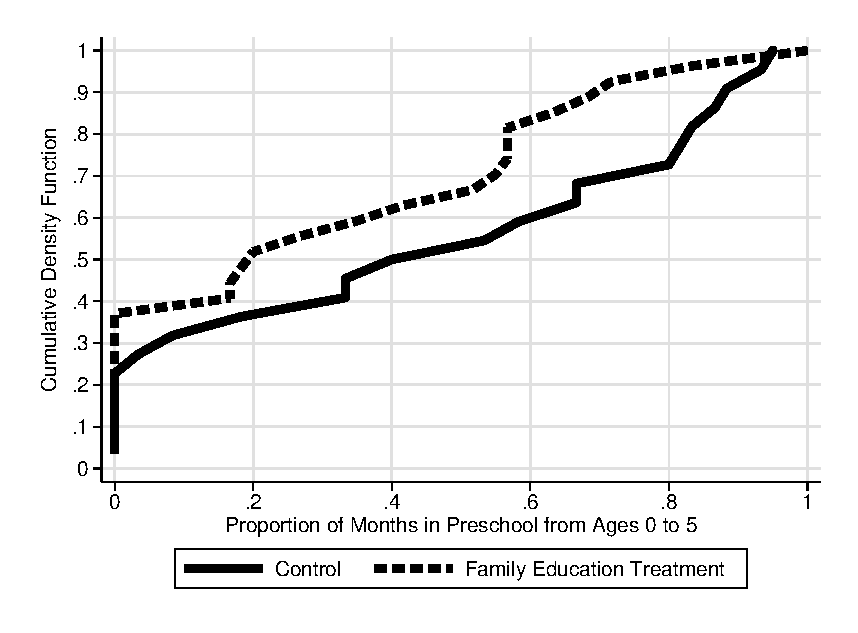
\includegraphics[width=.9\columnwidth]{output/care_controlcontamination_months.eps}
\floatfoot{
\footnotesize
\noindent Note: This figure displays the cumulative density function of enrollment in alternative preschools of the control and family education treatment groups in CARE.}
\end{figure}

\subsection{Program Costs} \label{section:programscosts}

The costs of the programs are a fundamental input to our calculations of the benefit-to-cost ratio and the internal rate of return. We improve on previous estimates of the costs by using primary-source documentation---progress reports written by the principal investigators and related documentation we recovered in the archives of the research center where the program was implemented. We display these sources in Appendix \ref{app:programcosts}.

Table~\ref{tab:totalcosts} breaks down the costs by different categories and items for a year of treatment. We obtain the personnel wages from the primary sources we show in Appendix \ref{app:programcosts} and include the type of personnel based on conversations with the programs' staff. Our sources display the actual wages without accounting for fringe benefits. We add 15\% to the wages to account for fringe benefits. The costs we label as ``other'' account for nutrition and services that the subjects  received when they were sick, diapers during the first 15 months of their lives, and transportation to the center.\footnote{The control children also received diapers during approximately 15 months, and iron-fortified formula. We assume that this generated a cost of half that amounts to half of ``other'' category for the first 15 months of their lives.} The costs are based on sources describing ABC treatment for $52$ children. We use the same costs estimates for the comparable CARE, for which information is less available.\footnote{CARE's treatment group that is relevant to our calculations, the center-based childcare and family education treatment group, received an additional service if compared to the treatment group in ABC: family education. The primary sources that we use indicate that this resulted in no additional cost. The staff implementing the center-based childcare treatment implemented the home visits without receiving an additional payment for doing so. We assume that any transportation costs to the children's home were minimal.}

\begin{table}[H]
\begin{threeparttable}
\caption{Yearly Program Costs, ABC and CARE} \label{tab:totalcosts}
\footnotesize
\begin{tabular}{lc} \toprule
\multicolumn{1}{c}{Item} & Yearly Cost in 2014 USD \\ \midrule
1 Program Director & $60,935$ \\ 
1 Social Worker      &  $35,869$ \\ 
3 Lead Teachers and 2 Teachers Aides (Nursery)  & $204,457$ \\
4 Lead Teachers and 4 Teacher Aides  (Toddlers) & $305,181$ \\ 
2 Teaching Support Staff & $53,341$ \\ 
1 Secretary & $32,973$ \\ 
1 Clerk        & $32,537$ \\ 
Workers' Fringe Benefits & $124,935$ \\ 
Other & $4, 891$ \\ \\ \midrule 
Total  & $962,726$ \\ 
Total per Subject & $18,514$ \\ \bottomrule
\end{tabular}
\begin{tablenotes}
\footnotesize
\item Sources: See Appendix~\ref{app:programcosts}.\\
\item Note: This table summarizes the yearly costs for ABC and CARE. They are based on primary-source documentation describing ABC. We assume that the costs for ABC and CARE were the same based on conversations with programs' staff \citet{projectcare2014interviews,abc2014-2015interviews}.
\end{tablenotes}
\end{threeparttable}
\end{table}

The costs exclude research-related or policy-analyses expenses. Our calculation amounts to $\$295,239$ (1979 USD). Notably, a completely independent calculation reported in \citet{FPG_1979_Progress-Report} indicates that the yearly cost of the program was $\$275,475$  (1979 USD). Although the calculations might have been based on the same primary sources, \citet{FPG_1979_Progress-Report} does not provide a break down of the costs.

\subsection{Non-experimental Data Sources}

Our cost-benefit analysis requires (i) \textit{interpolation} of components we do not observe due to intermittent data collection; and (ii) \textit{extrapolation} or forecasting of components we do not observe because the follow-ups stop when the subjects were in their mid-30s. We use multiple sources of non-experimental data representative on the national or state level to construct these interpolations and extrapolations. Table~\ref{table:sources} details the components for which we do these exercises and the sources we use. Section~\ref{section:methodology} explains our methodology for doing so.

\begin{table}[H]
\begin{threeparttable}
\caption{Auxiliary Data Sources for Interpolation and Extrapolation of Life-Cycle Benefits and Costs, ABC and CARE} \label{table:sources}
\footnotesize
%\input{../../AuxilliaryFiles/Preamble}
%\newgeometry{margin=.1in}

%\newcolumntype{L}[1]{>{\raggedright\let\newline\\\arraybackslash\hspace{0pt}}m{#1}}
%\newcolumntype{C}[1]{>{\centering\let\newline\\\arraybackslash\hspace{0pt}}m{#1}}
%\newcolumntype{R}[1]{>{\raggedleft\let\newline\\\arraybackslash\hspace{0pt}}m{#1}}

\begin{tabular}{L{3cm} C{1cm} C{1cm} C{1cm} C{1cm} C{1cm} C{2cm}} \toprule
 & \multicolumn{6}{c}{Subject's Age} \\
\textbf{Component}  & 16--21 & 21--30 & 31--34 & 34--50 & 61--67 & 68--Death \\ \midrule
\textbf{Transfer Income} & & \multicolumn{1}{c}{\cellcolor[gray]{.8} cNLSY} & \multicolumn{3}{c}{\cellcolor[gray]{.7} NLSY79; PSID}  &  \\ \midrule
\textbf{Subject Income} & &  \multicolumn{1}{c}{\cellcolor[gray]{.8} cNLSY} & \multicolumn{3}{c}{\cellcolor[gray]{.7} NLSY79; PSID} & \\ \midrule
\textbf{Health}  & \multicolumn{6}{c}{\cellcolor[gray]{.8} PSID; MEPS; MCBS; HRS}     \\ \midrule
\textbf{Crime} & \multicolumn{4}{c}{\cellcolor[gray]{.8} NCDPS; NJRP; NVS; UCRS} \\ \bottomrule
\end{tabular}
%\end{document}
\begin{tablenotes}
\footnotesize
Note: This table details the non-experimental data sources we use to interpolate and extrapolate the life-cycle benefits and costs of ABC and CARE. cNLSY: Children of the National Longitudinal Survey of the Youth 1979; NLSY79: National Longitudinal Survey of the Youth 1979; PSID: Panel Study of Income Dynamics; MEPS: Medical Expenditure Panel Survey; MCBS: Medicare Current Beneficiary Survey; HRS: Health and Retirement Study; NCDPS: North Carolina Department of Public Safety Data; NVS: National Crime Victimization Survey; NJRP: National Judicial Reporting Program; UCRS: Uniform Crime Reporting Statistics.
\end{tablenotes}
\end{threeparttable}
\end{table}

\section{Methodology} \label{section:methodology}

\subsection{Parameters of Interest and Policy Questions} \label{section:methodsquestions}

Random assignment to treatment alone does not guarantee that conventional treatment-effect estimates commonly used in the literature are able to answer policy-relevant questions. For an estimator to be useful in policy design, it should relate to a relevant parameter by clearly stating the counterfactual scenario to which the evaluated program is being compared. We define three parameters and link them to different policy questions.

Let $Y$ denote an outcome of interest. $D$ indicates whether or not the parents of the subject agree to participate of the program and $R | D = 1$ denotes randomization to either treatment or control status; $T$ denotes the number of periods during the first phase of treatment---5 years.\footnote{We define parameters that are conditional on the parents agreeing to participate of the program. That is, conditional on $D = 1$. We find little sensitivity to the few cases of non-compliance in Appendix~\ref{appendix:assessingcc} and adjust our estimates for the cases of attrition as we explain in Appendix~\ref{appendix:attrition}.} We think of two counterfactuals under control status:
\begin{eqnarray}
Y_H^0 \left( t, \omega \right) &:& \textbf{ Outcome under control status; subject stays at home in period $t$} \nonumber \\
Y_C^0 \left( t, \omega \right) &:& \textbf{ Outcome under control status; subject attends preschool in period $t$}  \nonumber
\end{eqnarray}

We define the proportion of months in alternative preschool as
\begin{equation}
V \left ( \omega \right) : = \frac{\# \{ t: Y_H^0 \left( t, \omega \right) - Y_C^0 \left( t, \omega \right) \leq 0 \} }{T}.
\end{equation}

Describing the dynamic choices underlying $V \left ( \omega \right)$ is of interest but goes beyond the scope of this paper. We simplify the analysis by assuming that timing is irrelevant:
\begin{align}
Y_H^0 \left( t, \omega \right) &= Y_H^0 \left( \omega \right) \nonumber \\
Y_C^0 \left( t, \omega \right) &= Y_C^0 \left( \omega \right).
\end{align}
\textbf{[JJH: All programs alike]} The counterfactual outcome when the child is in control status is
\begin{equation}
Y^0 \left( \omega \right) : = \left[ 1 - V \left( \omega \right) \right] Y_H^0 \left( \omega \right) + \left[ V \left( \omega \right) \right] Y_C^0 \left( \omega \right),
\end{equation}
and make explicit its dependence on $V \left( \omega \right)$, allowing us to answer policy-relevant questions. Likewise, we write the outcome when the child is fixed to treatment status as $Y^1 \left( \omega \right)$.

There are two possible approaches. One approach is to treat $V \left( \omega \right)$ as binary, where $V \left( \omega \right) = 0$ or $V \left( \omega \right)  > 0$. The other approach is to allow for multiple values of $V$ and let $V$ to be continuous in the limit. The latter approach is ideal, because it would allow us to construct the counterfactual $Y_C^0 \left( v,  \omega \right) $ for $v \in [0 , 1]$ denoting a realization of $V$. This approach, however, is problematic in the context of the small number of observations in our experimental datasets. While the former approach limits the cases to either $V \left( \omega \right) = 0$ or $V \left( \omega \right)  > 0$, it still allows for the definition of policy-relevant parameters. Under this approach, we can frame the parental decision in a standard Roy-type setting noting that
\begin{equation}
\Pr \left[ Y^1 \left( \omega \right) \geq \max \left(  Y_{H}^0 \left( \omega \right) ,  Y_{C}^0 \left( \omega \right)   \right) \right] = 1, \label{eq:noutility}
\end{equation}
where we could also frame the problem in terms of parental utility function $U \left( \cdot \right) $ over the outcome $Y$. We present estimates for different versions of this Roy model in Appendix~\ref{appendix:amethodology}.

We focus on simpler parameters that we can directly use in the cost-benefit analysis. The estimates of these parameters and the Roy-model equivalents are qualitatively similar. The first parameter of interest relates to the following question: what is the effect of the program as implemented? That is, what is the effect of the program without fixing the parental decision of whether or not to enroll the subject in alternative preschool? Importantly, this parameter does not speak to the effectiveness of the program by itself. Instead, it speaks to the effectiveness of the program relative to the supply of alternatives preschools that was in place when the program was implemented. The parameter is:

\begin{equation}
\Delta := \mathbb{E}_{\Omega} \left[ Y^1 \left( \omega \right) -  \max \left(  Y_{H}^0 \left( \omega \right) ,  Y_{C}^0 \left( \omega \right)  \right) | D =1 \right]. \label{eq:mainest}
\end{equation}

Random assignment to either the treatment or control group allows us to identify this parameter.

It is perhaps more policy-relevant to inquire on the efficiency of a program with respect to a clearly stated counterfactual. For example, if we ask: what is the effectiveness of the program with respect to a counterfactual in which the child stays at home? The parameter associated with this question is:
\begin{equation}
\Delta \left( v = 0 \right) : =   \mathbb{E}_{\Omega} \left[ Y^1 \left( v, \omega \right) - Y^0 \left( v, \omega \right) | V = 0, D = 1 \right]. \label{eq:par0}
\end{equation}

Random assignment to the treatment group does not directly identify this parameter.\footnote{We abuse notation to index the realization of $V \left( \omega \right)$. Differently from the definition above, the first argument in $Y^r \left( \cdot, \cdot \right)$ represents the proportion of time in preschool alternatives and not a time period. We do this to avoid further complicating the indices of the counterfactual outcomes.} We can approximate it with the following estimator: \textbf{[JJH: Confuses estimator]}
\begin{equation}
\widehat{\Delta} \left( v = 0 \right) : = \widehat{\mathbf{E}} \left[ Y | R = 1, V \in \left[ 0 , \eta \right], D = 1 \right] - \widehat{\mathbf{E}} \left[ Y | R = 0, V \in \left[ 0 , \eta \right], D = 1 \right] \label{eq:estimates0}
\end{equation}
with $\eta \rightarrow 0$ and where $\widehat{\mathbf{E}}[\cdot]$ represents an estimate of $\mathbb{E}[\cdot]$. That is, we compare the subjects randomly assigned to treatment with the subjects randomly assigned to control in a neighborhood where subjects do not take preschool alternatives. Various matching estimators allow us to estimate how likely subjects are to take preschool alternatives, based on observed characteristics \citep{Heckman_Ichimura_etal_1997_REStud,Heckman_Ichimura_etal_1998_REStud}. We provide different versions of these estimators below.

Similarly, we define a parameter that allows us to compare the effectiveness of the program relative to the preschool alternatives:
\begin{equation}
\Delta \left( v > 0 \right) : =   \mathbb{E}_{\Omega} \left[ Y^1 \left( v, \omega \right) - Y^0 \left( v, \omega \right) | V > 0, D = 1 \right] \label{eq:par1}
\end{equation}
and provide an estimate analogous to \eqref{eq:estimates0}. The parameters in \eqref{eq:par0} and \eqref{eq:par1} address control substitution, in the sense that they fix the counterfactual comparison accounting for the decisions that the parents make to enroll children in alternative preschools.

\subsection{Testing Multiple Hypotheses}  \label{section:counts}

We are interested in the effects that the program has on multiple dimensions of human development. We have measures of outcomes from very early in life to the mid-30s. This generates a multiple hypothesis testing problem. Two approaches are: (i) adjust the inference to account for the correlation of the outcomes using a step-down procedure \citep{Lehman_Romano_2005_AnnStat,Romano_Shaikh_2006_AnnStat}; and (ii) monetize the outcomes to produce a cost-benefit analysis. We adjust the inference when estimating the parameters in Section~\ref{section:methodsquestions} as in \citet{Lehman_Romano_2005_AnnStat} and \citet{Romano_Shaikh_2006_AnnStat} and provide a cost-benefit analysis below. In this section, we provide an intermediate alternative that informs on the relative importance of different outcomes in the cost-benefit analysis.

Let $\mathcal{G}$ be the index set for different groups of outcomes and let $\mathcal{O}_{g}$ be a group of outcomes, with $g \in \mathcal{G}$. Let $F_{j,g}^R \left( y_{j,g}^R \right) $ be the marginal distribution of outcome $j$ in group $g$ when randomized into treatment $R = 1$ or control $R = 0$. Assume that we want to perform inference on estimates of parameters of the type \eqref{eq:mainest} across multiple outcomes. That is, inference on

\begin{equation}
\Delta_{j,g} := \mathbb{E}_{\Omega} \left[ Y_{j,g}^1 \left( \omega \right) -  \max \left(  Y_{j,g,H}^0 \left( \omega \right) ,  Y_{j,g,C}^0 \left( \omega \right)  \right) | D =1 \right].
\end{equation}
for the group of outcomes in $\mathcal{O}_{g}$. We want to test the null hypothesis
\begin{equation}
H_{0} : F_{j,g}^0 = F_{j,g}^1, \ \forall \ j \in \mathcal{O}_{g}.
\end{equation}

In practice, we test the hypothesis
\begin{equation}
H_{0} : \Delta_{j,g} = 0, \ \forall \ j \in \mathcal{O}_{g}.
\end{equation}

We use the following statistic to test this hypothesis:
\begin{equation}
T_{g} = \sum _{j=1}^{\# \mathcal{O}_g} \mathbf{1} \left[ \widehat{\Delta}_{j}^{g} > 0\right]. \label{eq:count}
\end{equation}

For inference purposes, we bootstrap this procedure and construct a null distribution. The $p$-value for the number of socially positive treatment effects in group $g$ is $1 - \widehat{F}_{g} \left( T_{g} \right)$, where $ \widehat{F}_{g}$ is the empirical bootstrap distribution of group $g$.\footnote{For the case where we count the number of positive and significant outcomes, we use a ``double bootstrap'' to produce an inference on the count. We resample $B_{0}$ times to obtain the $p$-value for testing the hypothesis of interest for each individual outcome. This allows us to compute the number of positive and significant treatment effects, for example. We repeat this procedure $B_{1}$ times to obtain a distribution for this count. Thus, the double bootstrap consists of $B_{0} \times B_{1}$ data resamplings.}

A particular case is to count the positive treatment effects in the outcomes across all the groups indexed in the set $\mathcal{G}$. This allows us to avoid (i) arbitrarily picking outcomes that have statistically significant effects---``cherry picking''; or (ii) arbitrarily blocking sets of outcomes to correct the $p$-values when accounting for multiple hypothesis testing.

We provide inference on this count and on a count of treatment effects that are both positive and significant for which the inference is analogous. We also provide counts for the parameters that account for control substitution.

\subsection{Forecasting and Monetizing Life-cycle Costs and Benefits} \label{section:cbamethodology}

\subsubsection{Treatment Effects} \label{section:teresults}

We consider \noutcomes\ measures of human development across the life cycle and count the measures for which the program had a ``socially positive'' effect, without accounting for control substitution.\footnote{These outcomes directly relate to the categories we monetize in the cost-benefit analysis. We analyze a more thorough list of outcomes in Appendix~\ref{appendix:moreoutcomes}. The results weaken, but not to a great extent. This is a consequence of adding outcomes for which it is not clear that treatment should have a positive treatment effect.} We do this for both ABC and CARE by focusing on the first phase of treatment to compare subjects who received center-based childcare to control-group subjects---noting that assignment was random.\footnote{In ABC, this implies comparing the subjects who were randomly assigned to the treatment group to the subjects who were randomly assigned to the control group, in the first phase. In CARE, this implies comparing the subjects who were randomly assigned to receive center-based childcare and family education to the subjects who were randomly assigned to the control group, in the first phase as well.} Figure~\ref{fig:ppositive} displays the results from this exercise: ABC and CARE positively impact a large percentage of the outcomes we consider.\footnote{The calculation of the standard errors follows from the bootstrap procedure we discuss in Section~\ref{section:methodology}.}

We can further decompose the counts in Figure~\ref{fig:ppositive} into arbitrary categories. To economize space, we present this exercise pooling ABC and CARE. That is, we decompose the effects described in the last two bars of Figure~\ref{fig:ppositive}. Figure~\ref{fig:ppositivecategory1} and Figure~\ref{fig:ppositivecategory2} present this exercise. This helps us better understand the type of outcomes the programs affected. The results indicate that a large and precise fraction of effects are positive for outcomes spanning the life cycle, from parental income to crime and including a wide variety of health categories.

Next we present an overview of outcome-specific results. Appendix~\ref{appendix:results} displays an extensive summary of the estimates for the \noutcomes\ outcomes we consider. Note that: (i) we arbitrarily pick the outcomes we discuss next because we consider them of economic interest; and (ii) Appendix~\ref{appendix:results} displays results accounting for multiple hypothesis testing as in \citet{Lehman_Romano_2005_AnnStat} and \citet{Romano_Shaikh_2006_AnnStat}. We do not lose significance in the majority of outcomes.

\begin{figure}[H]
		\caption{Positively Impacted Outcomes, ABC and CARE} \label{fig:ppositive}
		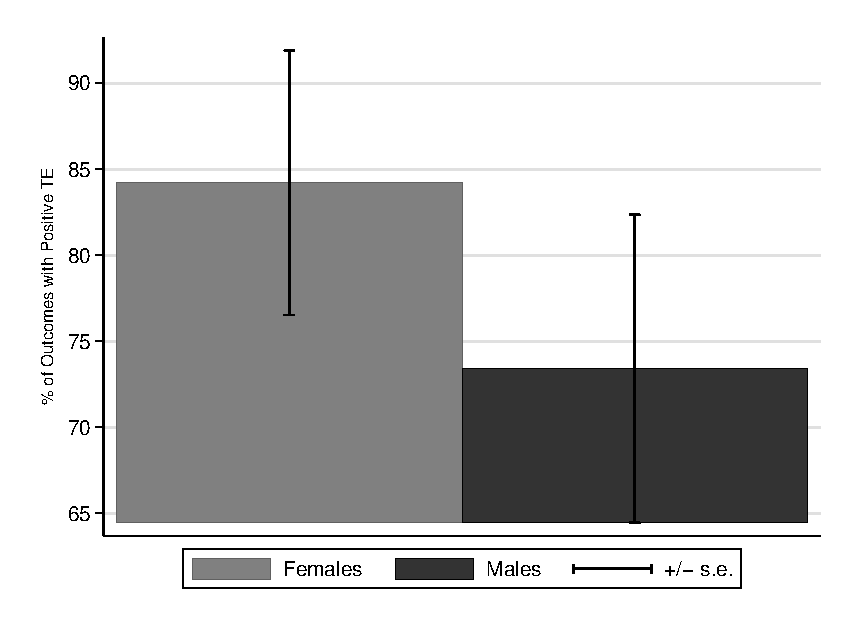
\includegraphics[width=.7\columnwidth]{output/itt_noctrl_all.eps}
\floatfoot{
\footnotesize
\noindent Note: The bars compare the mean of positive impacted outcomes between subjects in ABC and CARE who received center-based childcare and family education and subjects who receive either family education or no treatment at all.}
\end{figure}

To link the results thus far to the cost-benefit analysis of the programs, we monetize the treatment effects. At each age, we calculate each of the parameters assessing the counterfactuals of interest and monetize them, as we explain in Section~\ref{section:methodology}. We provide their life-cycle accumulated net present values. Thus, for each component we obtain the net present value of its contribution to the social benefit of the programs. To calculate the net present value, we first compare the treatment to the control group. The net present value represents the benefit (or cost) to the treatment group net of the benefit (or cost) to the control group. We then calculate the net present values accounting for control substitution.

\begin{figure}[H]
		\caption{Positively Impacted Outcomes by Category, ABC and CARE} \label{fig:ppositivecategory1}
		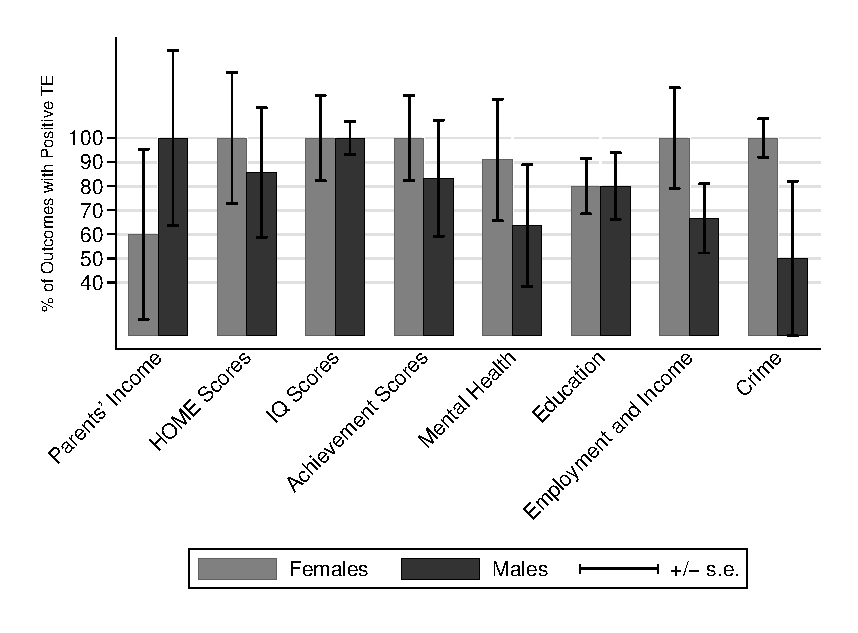
\includegraphics[width=.8\columnwidth]{output/itt_noctrl_cats1.eps}
\floatfoot{
\footnotesize
\noindent Note: For each outcome category, we compare the mean of the subjects who received center-based childcare in ABC and center-based childcare and family education in CARE to the mean of the subjects in the control group in both programs and count the number of positive comparisons.}
\end{figure}

\begin{figure}[H]
		\caption{Positively Impacted Health Outcomes, ABC and CARE} \label{fig:ppositivecategory2}
		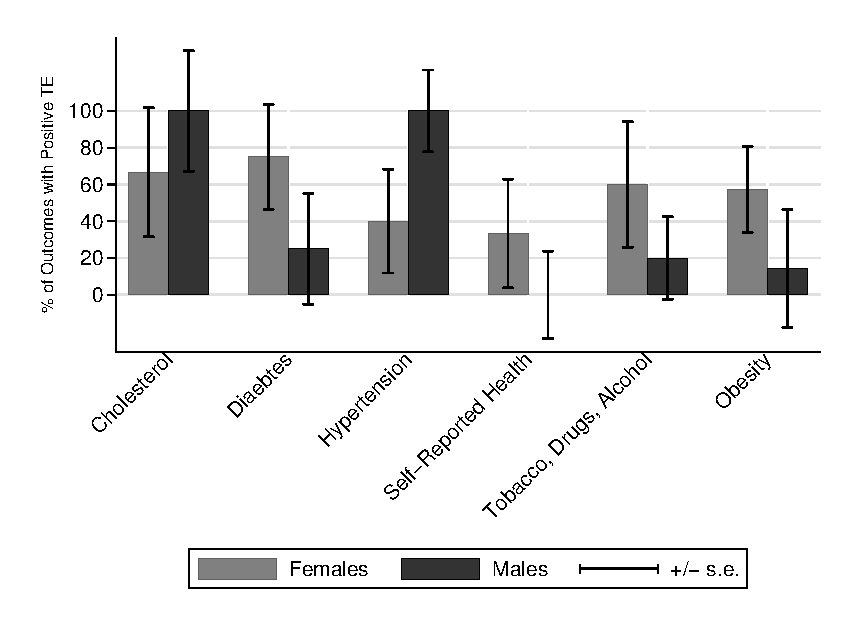
\includegraphics[width=.78\columnwidth]{output/itt_noctrl_cats2.eps}
\floatfoot{
\footnotesize
\noindent Note: For each outcome category, we compare the mean of the subjects who received center-based childcare in ABC and center-based childcare and family education in CARE to the mean of the subjects in the control group in both programs and count the number of positive comparisons.}
\end{figure}

Figure~\ref{figure:npvs} presents the net present values for the main components of the cost-benefit analysis pooling males and females. The ``Baseline'' bars represent the estimates based on the first parameter of interest, comparing the treatment- to the control-group children. The ``Stay at Home'' bars represent the comparison between the treatment group and the control group children who stay at home. The ``Alternative Preschool'' bars represent the comparison between the treatment group and the control-group children who attend alternative preschools.

We start by describing the components and the net present values for the baseline, treatment-control comparison.

The first category represents the cost of the programs' implementation. The second category quantifies the amount spent on control-group children in preschool alternatives. This is a benefit in the sense that parents of the treatment-group children did not spend money on preschool alternatives. Education costs are the third category and their net present value is negative because children in the control group acquired more education throughout their life cycles.

Labor income has two components. First, the parents of the treatment-group children increased their labor supply and therefore their income. This came as a consequence of being able to drop their children off at the treatment center for between four and eight hours a day for five years. The net present value we present span the first 15 years of the treatment and control children. Second, the program produces a positive net present value on labor income of the treated children. This considers the income from age 21 all the way to retirement.

We present three main categories for health. As we more extensively report in the Appendix and as documented in \citet{Campbell_Conti_etal_2014_EarlyChildhoodInvestments}, ABC and CARE had substantial effects on several measures of long-term health, especially for males---e.g. body-mass index, systolic and diastolic pressure, Framigham risk index. This translates into a higher probability of survival at later ages---we document this further in Appendix~\ref{appendix:health}. Thus individuals in the treatment group incur higher medical costs. However, their health conditions enable them to lead higher quality lives, which is reflected in the net gain the program generates in the quality-adjusted life years. Finally, crime is an important component. This is consistent with previous analysis of early childhood education programs \citep{Heckman_Moon_etal_2010_RateofReturn}. We analyze the internal rate of return and cost-benefit ratio implied by these net present values next.

Before doing do, it is important to note that although the net present values from the three comparisons imply that ABC and CARE are socially beneficial, independently to control substitution, the magnitudes for some of the components do vary substantially. As we argue next, this has to do with the differences between females and males in the treatment effects that the program has. As Figure~\ref{figure:npvsf} and Figure~\ref{figure:npvsm} show, males benefit much more when the counterfactual scenario is to attend alternative preschools, while females benefit much more from the program when the counterfactual scenario is to stay at home.

\textbf{[JJH: Redraft all of these figures] [Typist: Jorge is working on this] [JLG: New figures below.]}

\begin{sidewaysfigure}[H]
\caption{Life-cycle Net Present Value of Main Components of the CBA, Pooled Sample of Males and Females}
\label{figure:npvs}
\centering
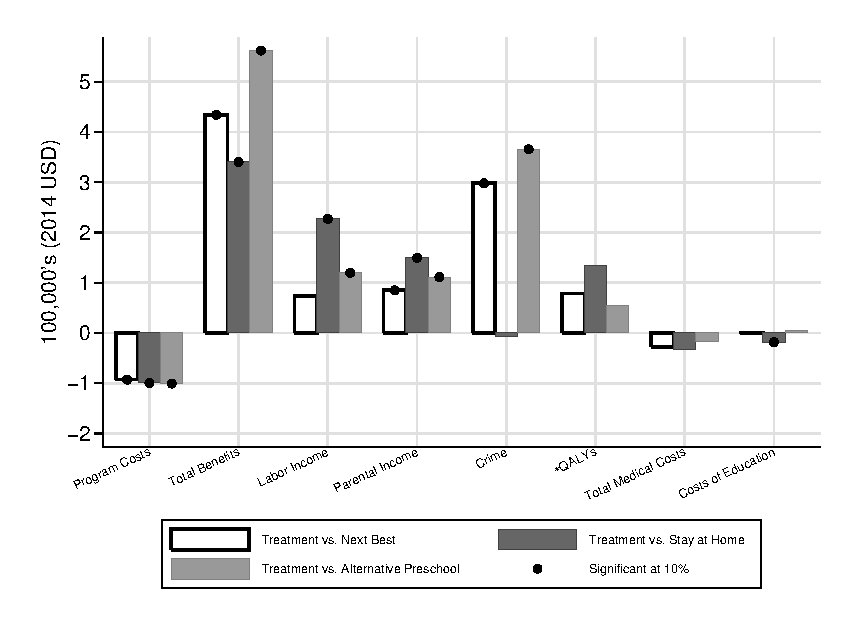
\includegraphics[width=.8\columnwidth]{output/abccare_npvs3.eps}
\floatfoot{
\footnotesize
Note: This figure displays the life-cycle net present value of the main components of the cost-benefit analysis of ABC and CARE. ``Treatment vs. Control'': compares the treatment to the control group. ``Treatment vs. Stay at Home'': compares the treatment group to those children who stay at home. ``Treatment vs. Alternative Preschool'': compares the treatment group to those children who attend alternative preschools. The latter two are based on matching estimators that account for selection on observable variables. By ``net” we mean that each component represents the total value for the treatment group minus the total value for the control group. Program costs refers to the total cost of implementing ABC/CARE. Total net benefits represents the total net benefits of \textit{all} the components we consider. Labor income represents total individual labor income from ages 20 to the retirement of program participants. Parental income represents total parental labor income of the parents of the program participants from when the participants were ages 0 to 15. Crime is the total cost of crime (judiciary plus victimization). QALYs refers to the quality-adjusted life years gain due to better health conditions through age 79. Total medical costs accounts for both private and public medical costs from ages 15 to 79. Costs of education represent the total costs of education of the individual from ages 6 to 26 and \textit{include any costs from special education and grade retention.}
}
\end{sidewaysfigure}

\begin{sidewaysfigure}[H]
\caption{Life-cycle Net Present Value of Main Components of the CBA, Females}
\label{figure:npvsf}
\centering
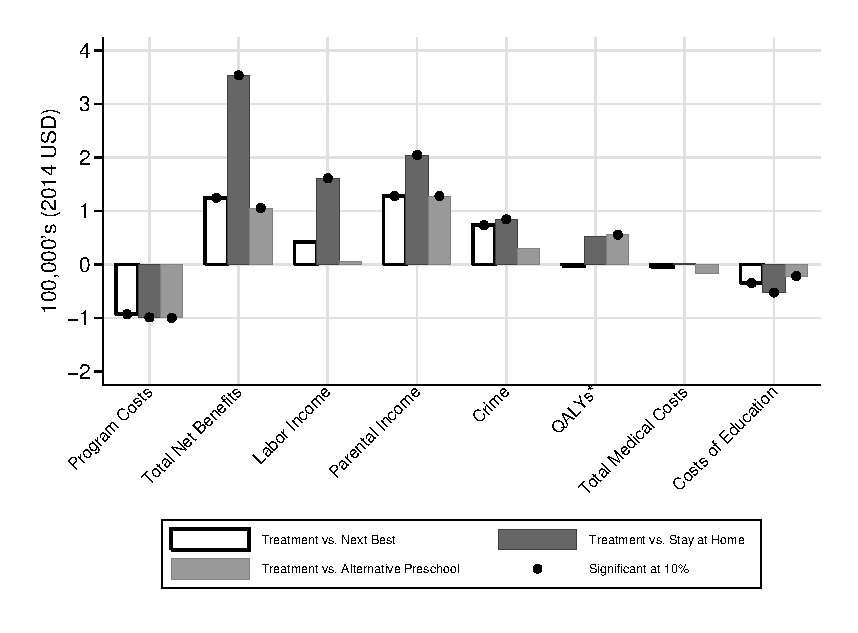
\includegraphics[width=.8\columnwidth]{output/abccare_npvs1.eps}
\floatfoot{
\footnotesize
Note: This figure displays the life-cycle net present value of the main components of the cost-benefit analysis of ABC and CARE. ``Treatment vs. Control'': compares the treatment to the control group. ``Treatment vs. Stay at Home'': compares the treatment group to those children who stay at home. ``Treatment vs. Alternative Preschool'': compares the treatment group to those children who attend alternative preschools. The latter two are based on matching estimators that account for selection on observable variables. By ``net” we mean that each component represents the total value for the treatment group minus the total value for the control group. Program costs refers to the total cost of implementing ABC/CARE. Total net benefits represents the total net benefits of \textit{all} the components we consider. Labor income represents total individual labor income from ages 20 to the retirement of program participants. Parental income represents total parental labor income of the parents of the program participants from when the participants were ages 0 to 15. Crime is the total cost of crime (judiciary plus victimization). QALYs refers to the quality-adjusted life years gain due to better health conditions through age 79. Total medical costs accounts for both private and public medical costs from ages 15 to 79. Costs of education represent the total costs of education of the individual from ages 6 to 26 and \textit{include any costs from special education and grade retention.}
}
\end{sidewaysfigure}

\begin{sidewaysfigure}[H]
\caption{Life-cycle Net Present Value of Main Components of the CBA, Males}
\label{figure:npvsm}
\centering
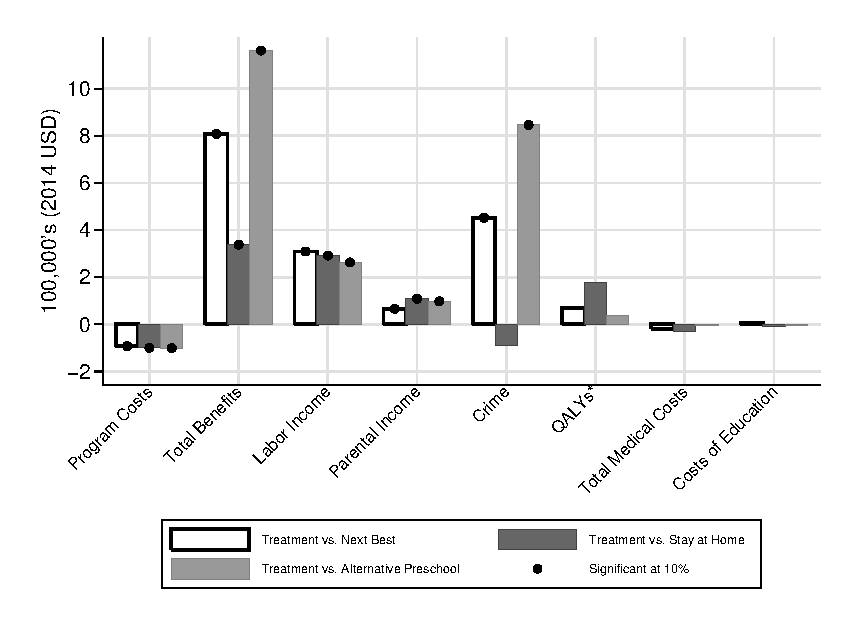
\includegraphics[width=.8\columnwidth]{output/abccare_npvs2.eps}
\floatfoot{
\footnotesize
Note: This figure displays the life-cycle net present value of the main components of the cost-benefit analysis of ABC and CARE. ``Treatment vs. Control'': compares the treatment to the control group. ``Treatment vs. Stay at Home'': compares the treatment group to those children who stay at home. ``Treatment vs. Alternative Preschool'': compares the treatment group to those children who attend alternative preschools. The latter two are based on matching estimators that account for selection on observable variables. By ``net” we mean that each component represents the total value for the treatment group minus the total value for the control group. Program costs refers to the total cost of implementing ABC/CARE. Total net benefits represents the total net benefits of \textit{all} the components we consider. Labor income represents total individual labor income from ages 20 to the retirement of program participants. Parental income represents total parental labor income of the parents of the program participants from when the participants were ages 0 to 15. Crime is the total cost of crime (judiciary plus victimization). QALYs refers to the quality-adjusted life years gain due to better health conditions through age 79. Total medical costs accounts for both private and public medical costs from ages 15 to 79. Costs of education represent the total costs of education of the individual from ages 6 to 26 and \textit{include any costs from special education and grade retention.}
}
\end{sidewaysfigure}


\subsubsection{Crime}  \label{sec:crime}

In this section, we explain how we quantify the benefits of the program from reductions in the subject's criminal activity. Two previous studies consider the impacts of ABC on crime: \citet{Clarke_Campbell_1998_ABC_Comparison_ECRQ} use administrative crime records up to age 21, and find no significant differences between the treatment and the control groups. \cite{Barnett_Masse_2007_EER} mention crime in their cost-benefit analysis, but they cite the previous study to claim that there are no savings coming from a reduction in crime. We consider richer data than the previous studies, which allows us to consider crime with a comprehensive life-cycle perspective: we gather various data sources, including administrative data on individual criminal records up to age 34, and project crimes until age 50 using prediction models based on local microdata.

We consider the following types of crime: arson, assault, burglary, fraud, larceny, miscellaneous (which includes traffic and non-violent drug crimes), murder, vehicle theft, rape, robbery, and vandalism. We use data from: (i) administrative youth arrests datasets, gathered for the age-21 follow-up; (ii) administrative adult arrests datasets, gathered around age 34; (iii) administrative sentences datasets, gathered around age 34; and (iv) self-reported adult crimes datasets, gathered in the age-21 and age-30 subject interviews. Because none of these data sources capture all criminal activity, it is necessary to combine them to more completely approximate the crimes the subjects committed. These datasets are discussed more extensively in Appendix \ref{appendix:crime}. The data are comprehensive and cover the full potential criminal career of subjects up to age 34, including details on the types of crimes and their timing, as well as projected and effective sentences.

We use several auxiliary datasets to construct national arrests-to-sentences and victims-to-arrests ratios: (i) the National Crime Victimization Survey (NCVS) to estimate the number of victims of crime; (ii) the National Judicial Reporting Program (NJRP) to estimate the number of sentences; and (iii) the Uniform Crime Reporting Statistics (UCRS) to estimate the number of arrests. Finally, we use microdata from the North Carolina Department of Public Safety (NCDPS) to estimate a prediction model for future crimes. This dataset contains information since 1972 on every individual who was convicted of a crime and entered the state prison system.

We follow four steps to estimate the costs of crime. We summarize the steps here and present a broader discussion in Appendix \ref{appendix:crime}.

\begin{enumerate}
\item \textit{Count arrests and sentences.} We start by counting the total number of sentences for each individual and type of crime (robbery, larceny, etc.) up to age 34. Then, we match the data on adult arrests, juvenile arrests, and self-reported crimes, to construct the total number of  arrests for each individual and type of crime up to that age.\footnote{In practice, we count all offenses (an arrest might include multiple offenses). This gives the correct number of victims for our estimations. The youth data have coarser categories than the rest of the data, so we assume that all property crimes were larcenies and that all violent crimes are assaults. In our sample, assault is the most common type of violent crime, and larceny/theft is the most common property crime.} About 10\% of the ABC and CARE samples have missing arrest data. For these cases, we impute the number of arrests by multiplying the number of sentences for each type of crime by the  national arrests-to-sentences ratio for the respective crime.
\item \textit{Construct predictions.} Based on the sentences observed before age 34, we predict the sentences that the ABC and CARE subjects will have after that age. The NCDPS data provide lifetime sentences of individuals in North Carolina, the same state in which the program was implemented. In that dataset, we estimate linear prediction models for each type of crime in which sentences after age 34 are the outcomes, and sentences up to age 34 are the regressors. Then, we apply these models to the ABC and CARE data. The outcome for each crime type is the number of future sentences for each subject, up to age 50. We assume that individuals with no criminal records before age 34 commit no crimes after age 34. We then add these estimates to the original number of sentences, getting an estimate of the lifetime sentences. To the best of our knowledge, no prior study on the benefits and costs of an educational program has used microdata to estimate a predictive model for future crimes. The predictions are an important component of total crime, as adding them increases the total count of crimes by 30\%--50\%. The prediction models we estimate and the results in terms of additional crimes are presented in Appendix \ref{appendix:crime}.
\item \textit{Estimate number of victims of crimes.} We observe crimes that resulted in consequences in the judicial system (i.e. crimes that resulted in arrests, sentences, or both). However, it is possible that for any subject for whom we observe to have committed a crime, he committed more crimes that we do not observe. Victimization inflation (VI) is a method to capture benefits of crime reduction for crimes without consequences in the judicial system that are unobserved in the ABC and CARE data. Previous papers using this method include \citet{Belfield_Nores_etal_2006_JHR} and \cite{Heckman_Moon_etal_2010_RateofReturn}. We start by constructing a VI ratio, which is the national ratio of victims-to-arrests for each type of crime.\footnote{We assume that each crime with victims is counted separately in the national reports on arrests, even for arrests that might have been motivated by more than one crime.} Then, we estimate the number of victims for each type of crime committed by ABC and CARE subjects as their total arrests multiplied by the VI ratio. Additionally, we can calculate an analogous estimate of the number of crime victims using sentences, based on the VI ratio and the national arrests-to-sentences ratio. Both estimates are very similar, as shown in Appendix \ref{appendix:crime}. To improve precision, the estimates in the rest of our paper are based on the average of the two.
\item \textit{Find total costs of crimes.} We use the estimates of the cost of crimes for victims from \cite{McCollister_etal_2010_DAD} to impute the total victimization costs (see Appendix \ref{appendix:crime} for details on the costs we use). For crimes having arrests, sentences, or both, we consider judicial system costs as well, such as police costs.\footnote{To be able to assign costs to each type of crime, we assume that the cost of the justice system depends on the number of offenses of each type, rather than on the number of arrests. While this could very slightly overestimate justice system costs, the costs only represent about 5\% of the total crime costs.} Finally, we construct the total costs of incarceration for each subject using the total prison time and the cost of a day in prison.
\end{enumerate}

\subsubsection{Health} \label{section:health}

We use an alternative methodology for health-related outcomes. There are three main reasons for this: (i) health outcomes such as diabetes or heart disease are absorbing states; (ii) health outcomes are highly interdependent within and across time; and (iii) there is no evident time period available to finish accounting for benefits and costs. For example, for income we extrapolate up to the retirement age of 67. However, for health, we need to predict an age of death for each individual. Thus, using the notation so far, it is not sufficient to condition on $W, Z, X$ to recover a credible estimate of the treatment effect. Instead, we use an adaptation of the Future America Model (FAM) that projects health outcomes from the subjects' early- to mid-30s up to their projected death \citep{Goldman_etal_2015_Future-Elderly-Model-Report}.\footnote{The simulation starts at the age in which we observe the subject's age-34 health follow-up. On average this happened at age 34 for both males and females, but there is variation ranging from age 30 to age 37.}

We provide a brief description of the model in this subsection. Appendix~\ref{appendix:health} provides a thorough discussion. The methodology has six steps: (i) estimate the age-by-age health state transition probabilities using the Panel Study of Income Dynamics (PSID); (ii) match these transition probabilities to the ABC and CARE individuals based on observed characteristics; (iii) estimate quality-adjusted life year (QALY) models using the Medical Expenditure Panel Survey (MEPS) and the PSID; (iv) estimate medical cost models using the MEPS and the Medicare Current Beneficiary Survey (MCBS), allowing estimates to differ by health state and observed characteristics; and (v) predict the medical expenditure and QALYs that correspond to the simulated individual health trajectories.\footnote{As an intermediate step between (i) and (ii), we impute some of the variables used to initialize the FAM models (see Appendix~\ref{appendix:health}}.

Our microsimulation model starts the health predictions at age 30, with the information on observed characteristics available at this age. We restrict it to the individuals for whom we have information from the age-34 health follow-up. This allows us to account for components that are crucial for predicting health outcomes, such as the body mass index (BMI). The models predict the probability of being in any of the states in the horizontal axis of Table~\ref{table:transition} at age $a+1$ based on the state at age $a$, which is described by the vertical axis of the table. The crosses indicate if being in a health a state at age $a$ is relevant for the estimation of the probability of being in a health state at age $a + 1$.\footnote{In practice, the predictions are based on two-year lags, due to data limitations in the auxiliary sources we use to simulate the FAM. For example, if the individual is 30 (31) years old in the age-30 interview, we simulate the trajectory of her health status at ages 30 (31), 32 (33), 34 (35), and so on until her projected dead.} Absorbing states are an exception. For example, heart disease at age $a$ does not enter in the estimation of transitions for heart disease at age $a+1$ because it is an absorbing state: once a person has heart disease, she carries it through the rest of her life. The same is true for chronic or permanent conditions such as hypertension, having a stroke, etc.

At each age, once we obtain the transition probability for each health outcome, we draw a Monte-Carlo simulations for each subject. Thus, each simulation depends on each individual's health history and on their particular characteristics. For every simulated trajectory of health outcomes, we predict the lifetime medical expenditure using the models estimated from the MEPS and the MCBS. We then obtain an estimate of the expected lifetime medical expenditure by taking the mean of each individual's simulated lifetime medical expenditure. The same procedure is applied to QALYs.

A quality-adjusted life year (QALY) reweighs a year of life according to its quality given the burden of disease. A QALY of 1 denotes a year of life in the absence of disease (perfect health). The value of QALY for an individual in a given year is smaller than 1 when there is positive burden of disease, as worse health conditions imply lower QALYs.\footnote{When an individual dies, her QALY equals zero. It is worth noting that there are extreme combinations of disease and disability that may generate negative QALYs, although this case is unusual.} We compute a QALY model based on the EQ-5D instrument, a widely-used Health-related Quality-of-life (HRQoL) measure, available in MEPS. We then estimate this model from the PSID. Appendix~\ref{appendix:health} provides more details on this estimation strategy.

\begin{sidewaystable}[H]
\begin{threeparttable}
\caption{Health State Transitions, Age $a$ as Predictor of Age $a+1$}\label{table:transition}
\scriptsize
\begin{tabular}{l|cccccccccccccc} \toprule
\multicolumn{1}{c}{Age $a$} & \multicolumn{14}{c}{Age $a+1$} \\ \midrule
  & Heart & Hyper- & Stroke & Lung  & Diabetes & Cancer & Disability & Mortality & Smoking  & Obesity & Health  & DI  & SS  & SSI  \\
&  Disease & tension &  & Disease & & & & &  &  & Insurance & Claim & Claim & Claim \\
Heart Disease & & & $\times$& & & &$\times$ &$\times$ & $\times$           &       &  $\times$  & $\times$ & $\times$ & $\times$\\
Hypertension  &  $\times$& & $\times$ & & & &$\times$ &$\times$ &       &     & $\times$   & $\times$ & $\times$  & $\times$\\
Stroke           & & & & & & &$\times$ &$\times$ &             &      &   $\times$  & $\times$ & $\times$  & $\times$\\
Lung Disease & & & & & & &$\times$ &$\times$ & $\times$         &        &   $\times$  &$\times$  & $\times$  & $\times$\\
Diabetes       & $\times$ &$\times$  & $\times$   & & & &$\times$ &$\times$ & $\times$            &       &  $\times$    & $\times$& $\times$ & $\times$ \\
Cancer         & & & $\times$ &  & &   &$\times$ & $\times$&           &         &   $\times$  & $\times$ & $\times$  & $\times$\\
Disability     & & & & & & &$\times$ &$\times$ &         &      &     $\times$  & $\times$ & $\times$   & $\times$\\
\midrule
Smoking & $\times$& $\times$&$\times$ & $\times$& $\times$& $\times$&$\times$ &$\times$ & $\times$   &   &     $\times$  & $\times$ & $\times$   & $\times$\\
BMI & $\times$& $\times$&$\times$ & $\times$& $\times$& $\times$&$\times$ & & $\times$    &  $\times$ &     &  &   & \\
Physical Activ. & $\times$& $\times$&$\times$ & $\times$& $\times$& $\times$&$\times$ & & $\times$    &   &     &   &  & \\
Binge Drinking & & & & & & &  &$\times$ & $\times$    &      &      &   &     &  \\
\midrule
DI Claim      & & & & &  & & & &             &         & $\times$    & $\times$   & $\times$ & $\times$\\
SS Claim     & & & & & & & &           &         &     & $\times$ &  & & $\times$\\
SSI Claim   & & & & &&  & & &         &        &      & &   & $\times$\\ \bottomrule
\end{tabular}

\begin{tablenotes}
\footnotesize
\item Note: This table illustrates how health outcomes at age $a$ predict health outcomes at age $a+1$. The crosses indicate if we use the age $a$ outcome to predict the age $a+1$ outcome. DI Claim: disability insurance claim; SS Claim: social security claim; DB Claim: disability benefits claim; SSI Claim: supplemental security income claim. The age $a$ states that do not predict themselves at age $a+1$ are absorbing states by construction.
\end{tablenotes}
\end{threeparttable}
\end{sidewaystable}

We estimate three models of medical spending: (i) Medicare spending (annual medical spending paid by parts A, B, and D of Medicare); (ii) out-of-pocket spending (medical spending paid directly by the individual); and (ii) all public spending other than Medicare. Each medical spending model is estimated through pooled weighted least squares regressions that include a person's demographics, economic status, current health, risk factors, and functional status as explanatory variables. The MCBS-based medical spending models also include lagged health because of the length of time for which MCBS subjects are observed.

\textbf{Medical Expenditure before Age 30}

We combine the MEPS and retrospective information in the ABC and CARE interviews at ages 21 and 30 related to hospitalizations at ages 12 and 15 and births at age 15. In addition to this retrospective information, we use use individual and family demographics to predict medical expenditure models for each age, as summarized in Table~\ref{table:pre30}.

\begin{table}[H]
\begin{threeparttable}
\caption{Health Expenditure Models by Age Group, before Age 30}\label{table:pre30}
\begin{tabular}{lcccc} \toprule
Explanatory variable & \multicolumn{4}{c}{Age Group} \\
& 8-11 & 12-14 & 15-20 & 21-30 \\
\midrule
Race/ethnicity & \checkmark & \checkmark & \checkmark & \checkmark \\
Education        & $\times$ & $\times$ & $\times$ & \checkmark \\
Asthma Diagnoses & \checkmark & \checkmark & \checkmark & \checkmark \\
Hospital stays & if $\geq$ 1 week & any stay & any stay & $\times$ \\
Births & $\times$ & $\times$ & \checkmark & \checkmark \\
Mother present & $\times$ & \checkmark & \checkmark & $\times$ \\
Father present & \checkmark & \checkmark & $\times$ & $\times$ \\
Number of siblings & \checkmark & \checkmark & $\times$ & $\times$ \\
Foodstamps & \checkmark & \checkmark & \checkmark & \checkmark \\
Living arrangements & $\times$ & $\times$ & \checkmark & \checkmark \\
Working, if working age & $\times$ & $\times$ & \checkmark & \checkmark \\
\bottomrule
\end{tabular}
\begin{tablenotes}
\footnotesize
\item Note: This table summarizes the explanatory variables included in the models we use to predict medical expenditure for each age group. Possible living arrangements are: living with parents, away at college, married, or other.\\
\end{tablenotes}
\end{threeparttable}
\end{table}

The first level of each model predicts the likelihood that the subject incurred any medical expenditure in the period. The second level predicts the medical expenditure for those with positive expenditures.

\section{Results} \label{section:results}

\subsection{Cost-benefit Analysis} \label{section:cbaresults}

Table~\ref{table:cba} summarizes the cost-benefit analysis of the programs without accounting for control substitution. All the money figures are in 2014 USD and are discounted to each child's birth age, unless otherwise specified.

Pooling males and females, the results indicate that the program is socially efficient: the baseline estimates for the internal rate of return and the benefit-to-cost ratio are \irrp\ and \bcp. The program generates a benefit of \bcp\ for every dollar spent on it. This is of particular importance because ABC and CARE were much more expensive than other early childhood education programs like Perry or Head Start \citep{Elango_Hojman_etal_2016_Early-Edu}---the treatment involved more services over a longer time period.

The internal rate of return and the benefit-to-cost ratio are robust to sensitivity exercises. First, we remove the component due to parental income. In practice, ABC and CARE had a childcare subsidy component because it allowed the mothers to work causing additional parental income. This component amounts to \parincomenpvp. Even after removing this component, the internal rate of return and benefit-to-cost ratio indicate social efficiency of the program and remain statistically significant.

Parental income and crime are the components for which the internal rate of return and the benefit-to-cost ratio are the most sensitive.\footnote{We do not account for treatment effects on parental income beyond age 15 because some children report to move out of their households as early as this age. This makes ambiguous the effects that parental income could have on the subjects after age 15.} The reason for the sensitivity to parental income is that the amount is substantial and it is not heavily discounted because it accumulates during the first $15$ years of the children's life. Although crime is subject to more discounting, the amount due to crime savings is large so removing it diminishes both the internal rate of return and the benefit-to-cost ratio.

The estimates are robust to individually removing the rest of the components, and in most cases remain statistically significant. This happens for one of either two reasons: (i) the effects are substantial but they are heavily discounted because they happen later in life---e.g. labor income; or (ii) the effects happen early in life but are not as substantial---as in the amount that the control-group parents pay for their children to attend alternative preschools.

Next, we analyze the estimates when splitting the sample by males and females. Some of the estimates lose significance due to the reduction of observations after splitting the sample by gender. The point estimates remain robust across  the sensitivity analysis.

For females, we observe consistency except for the case where we remove the parental income component. We can observe that the female sample is the main driver of parental income when comparing its net present value between females and males.

For males, the estimates are robust, similar to the female samples. An exception occurs when we remove the component corresponding to quality-adjusted life years. Although the cost-to-benefit ratio remains virtually unchanged, the internal rate of return is negative. In this case, the internal rate of return is actually uninformative: it is negative due to the fact that, when excluding the quality-adjusted life years, the net-benefit streams cross from negative to positive generating multiple roots. The interpretation of the internal rate of return when the net-benefit streams cross in unclear \citep{Arrow-Levhari_1969_EJ}.\footnote{This reinforces the importance of considering the quality-life improvement due to better health conditions.}

\begin{sidewaystable}[H]
\begin{threeparttable}
\caption{Cost-benefit Analysis of ABC and CARE, Summary}
\label{table:cba}
\centering
\begin{tabular}{l r r r r r r r r r}																			
\toprule																			
&       \mc{3}{c}{Females}      &       \mc{3}{c}{Males}        &       \mc{3}{c}{Pooled}       \\																			
\cmidrule(lr){2-4}      \cmidrule(lr){5-7}      \cmidrule(lr){8-10}																			
Removed Component       &       NPV     &       IRR     &       B/C     &       NPV     &       IRR     &       B/C     &       NPV     &       IRR     &       B/C     \\																			
\midrule																			
None	&	161,759	&	\textbf{10.1\%}	&	\textbf{2.61}	&	919,049	&	\textbf{14.7\%}	&	\textbf{10.19}	&	636,674	&	\textbf{13.7\%}	&	\textbf{7.33}	\\
	&		&	(6\%)	&	(0.73)	&		&	(4\%)	&	(2.93)	&		&	(3\%)	&	(1.84)	\\ \\
Parental Income	&	148,854	&	4\%	&	1.12	&	107,907	&	\textbf{11\%}	&	\textbf{9.10}	&	116,953	&	\textbf{9\%}	&	\textbf{6.17}	\\
	&		&	(2\%)	&	(0.65)	&		&	(3\%)	&	(2.92)	&		&	(3\%)	&	(1.87)	\\
Subject Labor Income	&	41,908	&	9\%	&	\textbf{2.21}	&	238,105	&	\textbf{13\%}	&	\textbf{7.75}	&	133,032	&	\textbf{13\%}	&	\textbf{6.03}	\\
	&		&	(6\%)	&	(0.66)	&		&	(5\%)	&	(2.23)	&		&	(4\%)	&	(1.77)	\\
Subject Transfer Income	&	419	&	\textbf{10\%}	&	\textbf{2.61}	&	-7,265	&	\textbf{15\%}	&	\textbf{10.26}	&	-4,372	&	\textbf{14\%}	&	\textbf{7.38}	\\
	&		&	(6\%)	&	(0.73)	&		&	(4\%)	&	(2.93)	&		&	(3\%)	&	(1.84)	\\
Subject QALY	&	42,102	&	9\%	&	\textbf{2.20}	&	106,218	&	\textbf{14\%}	&	\textbf{9.14}	&	87,181	&	\textbf{13\%}	&	\textbf{6.48}	\\
	&		&	(6\%)	&	(0.69)	&		&	(6\%)	&	(2.73)	&		&	(5\%)	&	(1.79)	\\
Medical Expenditures	&	-16,037	&	9\%	&	\textbf{2.77}	&	-42,038	&	\textbf{15\%}	&	\textbf{10.61}	&	-31,221	&	\textbf{14\%}	&	\textbf{7.65}	\\
	&		&	(6\%)	&	(0.76)	&		&	(3\%)	&	(2.89)	&		&	(3\%)	&	(1.85)	\\
Alternative Preschools	&	16,691	&	8\%	&	\textbf{2.45}	&	13,434	&	\textbf{14\%}	&	\textbf{10.05}	&	14,659	&	\textbf{12\%}	&	\textbf{7.19}	\\
	&		&	(5\%)	&	(0.73)	&		&	(4\%)	&	(2.92)	&		&	(3\%)	&	(1.84)	\\
Education Costs	&	1,457	&	\textbf{10\%}	&	\textbf{2.59}	&	-7,852	&	\textbf{15\%}	&	\textbf{10.26}	&	-4,518	&	\textbf{14\%}	&	\textbf{7.37}	\\
	&		&	(6\%)	&	(0.72)	&		&	(4\%)	&	(2.93)	&		&	(3\%)	&	(1.86)	\\
Crime Costs	&	31,668	&	10\%	&	\textbf{2.34}	&	638,923	&	\textbf{9\%}	&	4.08	&	450,368	&	\textbf{8\%}	&	\textbf{3.06}	\\
	&		&	(6\%)	&	(0.62)	&		&	(5\%)	&	(2.18)	&	&	(4\%)	&	(1.01)	\\ \\
Deadweight Loss	&		&	\textbf{18\%}	&	\textbf{3.83}	&		&	\textbf{19\%}	&	\textbf{15.38}	&		&	\textbf{18\%}	&	\textbf{11.01}	\\
	&		&	(12\%)	&	(1.04)	&		&	(6\%)	&	(4.35)	&		&	(5\%)	&	(2.79)	\\
0\% Discount Rate	&		&		&	\textbf{5.06}	&		&		&	\textbf{25.45}	&		&		&	\textbf{17.40}	\\
	&		&		&	(2.82)	&		&		&	(10.42)	&		&		&	(5.90)	\\
7\% Discount Rate	&		&		&	\textbf{1.49}	&		&		&	\textbf{3.78}	&		&		&	\textbf{2.91}	\\
	&		&		&	(0.32)	&		&		&	(0.79)	&		&		&	(0.59)	\\
\bottomrule																			
\end{tabular}																			

\begin{tablenotes}
\item Note: This table presents the estimates of the net present value (NPV) for each component, and the internal rate of return (IRR) and the benefit-to-cost ratio (B/C) of ABC for different scenarios based on comparing the groups randomly assigned to receive center-based childcare and the groups randomly assigned as control in ABC and CARE. The first row represents the baseline estimates. The rest of the rows present estimates for scenarios in which we remove the NPV estimates of the component listed in the first column. The quantity listed in the NPV columns is the component we actually remove when computing the calculation in each row. All the money figures are in 2014 USD and are discounted to each child's birth, unless otherwise specified. For the B/C we use a discount rate of $3\%$, unless otherwise specified. We test the null hypotheses $\text{IRR} = 3\%$ and $\text{B/C} = 1$---we elect $3\%$ because that is the discount rate we use. The results in bold are significant at the 10\% level in a single-sided, non-parametric, bootstrapped test. We resample both the experimental and the auxiliary data sources.
\end{tablenotes}
\end{threeparttable}
\end{sidewaystable}

Finally, we provide a cost-benefit analysis of the program when accounting for control substitution (Table~\ref{table:cbacs}). The first row shows the estimates without accounting for control substitution, i.e. the same as those of the first row in Table~\ref{table:cba}. The second and third rows present results for the two counterfactual comparisons we consider.

Before discussing the results, it is worth noting that the sample sizes for some of the cases make the IRR estimates very unstable. For example, the estimates for females compared to the counterfactual of staying at home are based on an initial sample of 5 observations in the control group, while the estimates for males are based on 7  observations in the control group.\footnote{That is, we observe 5 females and 7 males in the control group who did not attend alternative preschools. Some of the forecasts could be based on even smaller samples due to missing values in some specific outcomes.} In the specific case of females, the internal rate of return corresponding to the counterfactual of staying at home is based on crossing net-benefit streams. Similarly, we cannot obtain a real solution for the case of males.

The samples used to produce estimates relative to enrollment in alternatives preschools are larger than those previously mentioned and we are able to obtain real solutions for the IRR even after splitting by males and females. Despite these practical difficulties, the results are consistent with the treatment effects we show in Section~\ref{section:teresults}. Compared to ABC and CARE, females benefit more than males from alternative preschools relative to staying at home. That is, the benefit-to-cost ratio of ABC and CARE relative to staying at home is high for females and low for males. Conversely, the benefit-to-cost ratio of ABC and CARE relative to alternative preschools is high for males and low for females. Given the outcomes that we are able to monetize have higher values for males than for females, the pooled results are more similar to the results for males than to the results for females. Regardless, any of the counterfactual comparisons we consider indicates that ABC and CARE are socially efficient.

\textbf{[JJH: Table 8 --- get from Jorge] [Typist: Jorge is working on this]}

\begin{table}[H]
\begin{threeparttable}
\caption{Cost-benefit Analysis Accounting for Control Substitution, ABC and CARE}
\label{table:cbacs}
\centering
\begin{tabular}{l c c c c c c }
\toprule
	&	\mc{2}{c}{Females}					&	\mc{2}{c}{Males}					&	\mc{2}{c}{Pooled}					\\
		\cmidrule(lr){2-3}						\cmidrule(lr){4-5}						\cmidrule(lr){6-7}					
Estimate 	&	IRR	&	B/C	&	IRR	&	B/C	&	IRR	&	B/C	\\
\midrule

% INSERT summary_tex.xls FILE BELOW
% INSERT summary_tex.xls FILE BELOW
% INSERT summary_tex.xls FILE BELOW

Baseline	&	0.10 	&	\textbf{2.59}	&	\textbf{0.14} &	\textbf{9.75} 	&	\textbf{0.13}	&	\textbf{5.58}	\\
	&	(0.07)	&	(0.97)	&	(0.05)	&	(4.59)	&	(0.05)	&	(2.32)	\\
Relative to Staying at Home	&	\textbf{0.15}	&	\textbf{4.81}	&	\textbf{0.09}	&	4.32	&	\textbf{0.10} &	\textbf{4.42}	\\
	&	(0.07)	&	(1.42)	&	(0.04)	&	(2.70)	&	(0.03)	&	(1.39)	\\
Relative to Alternative Preschools	&	0.10		&	\textbf{2.37}	&	\textbf{0.17}	&	\textbf{12.38}	&	\textbf{0.14}	&	\textbf{6.29}	\\
	&	(0.07)	&	(0.91)	&	(0.05)	&	(5.16)	&	(0.04)	&	(2.23)	\\

% INSERT summary_tex.xls FILE ABOVE
% INSERT summary_tex.xls FILE ABOVE
% INSERT summary_tex.xls FILE ABOVE

\bottomrule
\end{tabular}
\begin{tablenotes}
\item Note: This table displays estimates of the internal rate of return (IRR) and the benefit-to-cost ratio (B/C) for ABC and CARE for three cases. Not accounting for control substitution (baseline); comparing ABC and CARE to staying at home (relative to staying at home); and comparing ABC to alternative preschools (relative to alternative preschools). For the B/C we use a discount rate of $3\%$. We test the null hypotheses $\text{IRR} = 3\%$ and $\text{B/C} = 1$---we elect $3\%$ because that is the discount rate we use. The results in bold are significant at the 10\% level in a single-sided, non-parametric, bootstrapped test. We resample both the experimental and the auxiliary data sources.
\end{tablenotes}
\end{threeparttable}
\end{table}


\section{Summary} \label{section:conclusion}

The evidence from policies related to early childhood education is still scarce despite its importance in the public debate. We provide a thorough evaluation of two randomized controlled trials: the Carolina Abecedarian Project (ABC) and the Carolina Approach to Responsive Education (CARE).

As programs providing high-quality center-based childcare, ABC and CARE have positive effects on a variety of outcomes measuring human development throughout childhood to adulthood---including cognition, socio-emotional skills, criminal activity, and adulthood health. This translates into statistically and economically significant measures of social efficiency, like the benefit-to-cost ratio and the internal rate of return, which we calculate accounting for complications that arise when evaluating social programs and considering life-cycle gains.

When adequately assessed, early childhood education programs enhance human development in that they provide a vehicle to promote social mobility. An adequate assessment requires: (i) comparing the program with respect to a well-defined counterfactual---e.g. other programs or staying at home; and (ii) monetizing the life-cycle gains, which goes beyond back-of-the-envelope calculations based on short-term gains.

\clearpage

%References
\singlespace
\bibliographystyle{chicago}
\bibliography{heckman}

\end{document} 